\documentclass[a4paper,11pt]{article}

\usepackage{graphicx}
\usepackage{amsmath}
\usepackage{enumitem}
\usepackage{blindtext}
\usepackage{tabularx}
\usepackage{multirow}
\usepackage{geometry}
	\geometry{
	margin = 1in
}
\usepackage{pdflscape}
\usepackage{fancyhdr}
	\pagestyle{fancy}
	\lhead{}
	\chead{}
	\rhead{}
	\lfoot{}
	\cfoot{}
	\rfoot{\thepage}
	\renewcommand{\headrulewidth}{0pt}
\usepackage[T1]{fontenc}
\usepackage[math]{iwona}
\usepackage{mathptmx}
\usepackage{titlesec}
\usepackage{longtable}
\usepackage{caption}
	\setlength{\abovecaptionskip}{0.5em}
\usepackage{makecell}
\usepackage{etoolbox}
	\apptocmd{\sloppy}{\hbadness 10000\relax}{}{}
\usepackage{setspace}
\usepackage{hyperref}
\usepackage{apacite}

\title{\Huge{ENG2016: Bike Project}}
\author{\begin{tabular}{l c}
		Ivan Mihajlovic&2239242 \\
		William Ely&2292204 \\
		Qiyu Zhang&2295435 \\
		Ewan Walker&2235937 \\
		Eduard Fiedler&2248902 \\
\end{tabular}
}
\date{2018}

\linespread{1.5}

\renewcommand{\contentsname}{Table of Contents}

\newcommand{\sectionbreak}{\clearpage}

\begin{document}

\pagenumbering{roman}

\begin{titlepage}

	\vspace*{\fill}
    	\begin{center}
		
\includegraphics[width=0.5\textwidth]{logo}\\
		\vspace{5em} 
		\hrulefill\\
		\vspace{0.8em} 
		\Huge{ENG2016: Bike Project}\\\hrulefill
		\vspace{2em}\\
		\LARGE{
			{\huge\textsc{Group 23}\vspace{2em}}\\
			\begin{tabular}{l c}
				Ivan Mihajlovic\phantom{W}&2239242 \\
				William Ely&2292204 \\
				Qiyu Zhang&2295435 \\
				Ewan Walker&2235937 \\
				Eduard Fiedler&2248902 \\
			\end{tabular}}\\
    	\end{center}
    	\vspace*{\fill}
	\vspace{10em} 

\end{titlepage}

\setcounter{page}{2}

\section*{Abstract}
\addcontentsline{toc}{section}{Abstract}

The purpose of this project was to design an electric bicycle for 55+ year-old men who want to commute to work without arriving sweaty. The report provides a detailed step-by-step walkthrough of the team's decisions made throughout the whole process. 

A decentralised organizational structure was used to aid the creation of ideas, and ensure that all problems had been tackled from several viewpoints. Once the fundamental infrastructures were estabilished, background research, a detailed product design specification, and a market analysis were conducted. These proved useful, as they defined a target price and provided a strategy to penetrate the market with the final design: creating a classic-looking e-bike aimed at the Dutch and German markets, which hold the greatest market share for e-bikes in Europe. Further research was conducted in fields concerning the involvement of muscles and posture, as well as a thorough morphological analysis. Finally, once all the basics had been approved the project continued into the detailed design where components and materials were selected. 

The final product is a visually appealing e-bike, made from an aluminium frame, incorporating a full Bosch electric drivetrain, and full suspension; whilst maintaining a competitive price at \textsterling 1,930, ensuring future growth and development.

\pagebreak

\begingroup
\tableofcontents
\endgroup

\pagebreak

\listoftables
\addcontentsline{toc}{section}{List of Tables}

\pagebreak

\listoffigures
\addcontentsline{toc}{section}{List of Figures}

\pagebreak

\pagenumbering{arabic}

\section{Introduction}

The brief chosen for this project was to design an: \textit{``Electrically assisted bike aimed at a healthy male commuter aged 55+ who does not want to come to work sweaty.''}

Electric bicycles, also referred to as e-bikes, are bicycles that are fitted with an electric motor which helps the user gain momentum. They make use of rechargeable batteries as a means of providing power, whilst keeping the user mobile. There are many different categories of e-bikes, such as: pedal assist, throttle on demand, speed pedelec, and electric moped \cite{ebr}. With a growing interest in battery powered transportation devices, the electric bicycle has experienced a worldwide, rapid growth in popularity since 1998 \cite{wein07}.

The design of an e-bike presented many interesting factors to be considered on top of the ones present in usual bike designs. Some of these included the selection and integration of an electric motor, and the positioning of the batteries as these tend to be quite bulky. Furthermore, the design brief offered guidelines which allowed for interesting alternatives when creating ideas for the product, and finalising the detailed design.

This report includes a step-by-step walkthrough of the design process for this project. This includes the initial establishment of leadership and organisation, the creation of key documents such as the product design specification and the house of quality, and finally the whole technical decision process for the detailed design.

\section{Project Planning}

From the beginning of the project, it was made clear that there was going to be no particular leader in the group. This would reduce concentrated stress onto one person, and required each member to be responsible. Therefore in order to remain organised, an initial Gantt chart was formulated. The Gantt chart allowed a visualisation of work allocations for the various topics that were required to complete the project. 

\subsection{Initial Work Allocations}

\begin{table}[!ht]
	\centering
	\caption{Initial Gantt chart}
	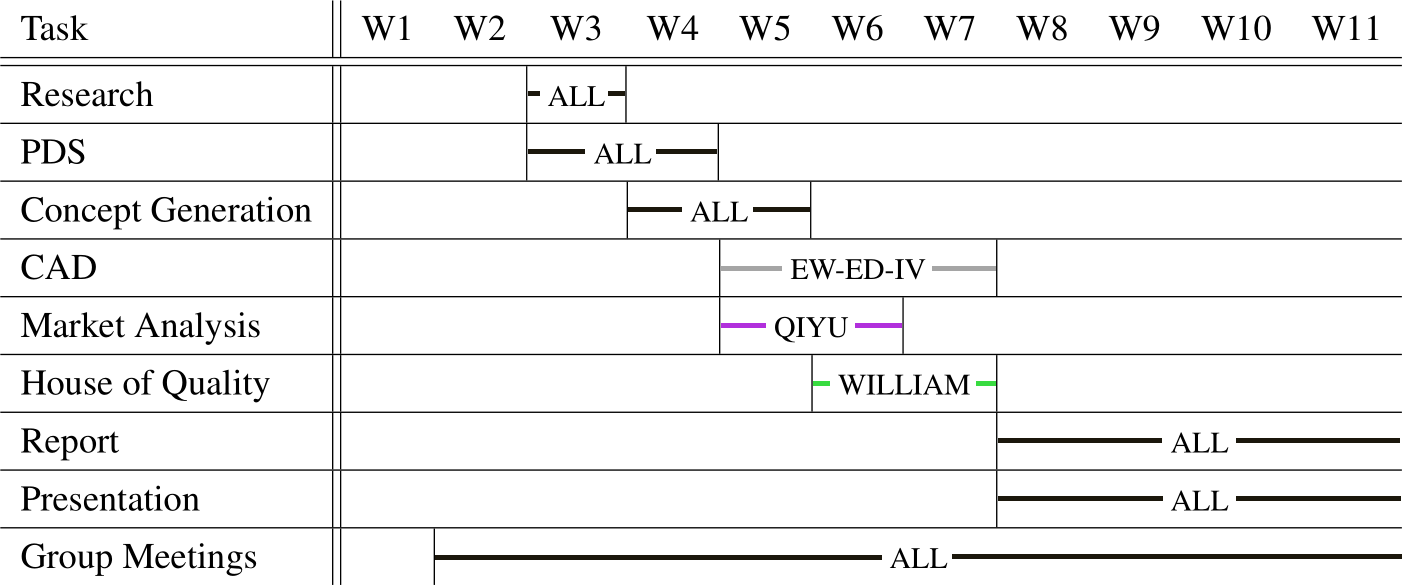
\includegraphics[width=1\textwidth]{gti}
	\label{tab:igc}
\end{table}

In terms of initial work distribution, each topic was allocated between the group members based on: background (course), experience from previous projects, and abilities. Therefore, Ewan, Eduard, and Ivan were assigned the CAD work, as William and Qiyu had little to no experience with SolidWorks. As a result, William and Qiyu were left to work on the Market Analysis and House of Quality.

The distribution of the CAD work was amongst 3 people, as it was speculated to take longer. Furthermore, in the initial stages group work (labelled `ALL') was emphasised to integrate individual concepts, and weekly group meetings were scheduled in order to remain on the same page.

\subsection{Final Work Allocations}
\label{sec:fwa}

As progress was made with the project, initial roles couldn't be maintained due to different individual schedules. Additionally, by further expanding on the generalised topics in the previous chart (Table~\ref{tab:igc}), the work had to be allocated differently. This resulted in the following work distribution in order to complete the project on time (see Tables~\ref{tab:gtc1} and~\ref{tab:gtc2}).

In the Final Gantt chart, the person to whom the Task is credited towards, is the one who contributed the most in that discipline. For example, in the process of producing the House of Quality, everyone contributed to the bulk of the decisions made at meetings. However, Eduard formulated the specifications from the PDS, further analysed the criteria, completed the diagram, and wrote the section for the report. Therefore, Eduard is credited in the chart, as he devoted the most time to the House of Quality. Every other task credited to one person, was completed in a similar manner.

Conversely, tasks completed by `ALL,' were completed by the entire group. This was achieved by either congregating in the form of a weekly group meeting and contributing to a task together; or creating an online document in which the group was able to gather and present their ideas.

In terms of milestones (Figure~\ref{fig:net}), initial research was concluded by week 5. Development into particular categories of the report was concluded in week 9. Further sections that had to be completed based on the previous milestone (e.g. Calculations, Costing, etc.) were completed in week 11. Afterwards, the body of work could then be analysed and was completed a week into the holidays (week 12). Following these milestones, the work was then compiled into a single document, and was further discussed by the entire group over the holidays. This allowed for the project to be completed on time.

\vspace{0.5em}
\begin{figure}[ht]
	\centering
	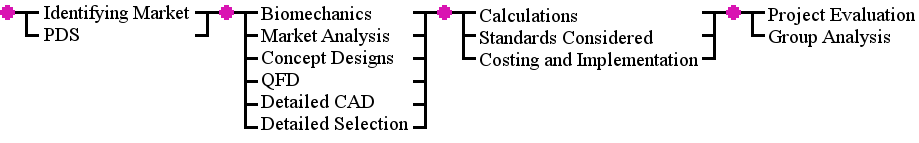
\includegraphics[width=0.98\textwidth]{milestone}
	\caption{Network diagram with milestones}
	\label{fig:net}
\end{figure}

\newgeometry{margin=0.8cm}
\thispagestyle{empty}
\begin{landscape}

\vspace*{\fill} 
\begin{table}[!ht]
	\centering
	\caption{Gantt Chart Weeks 1-6}
	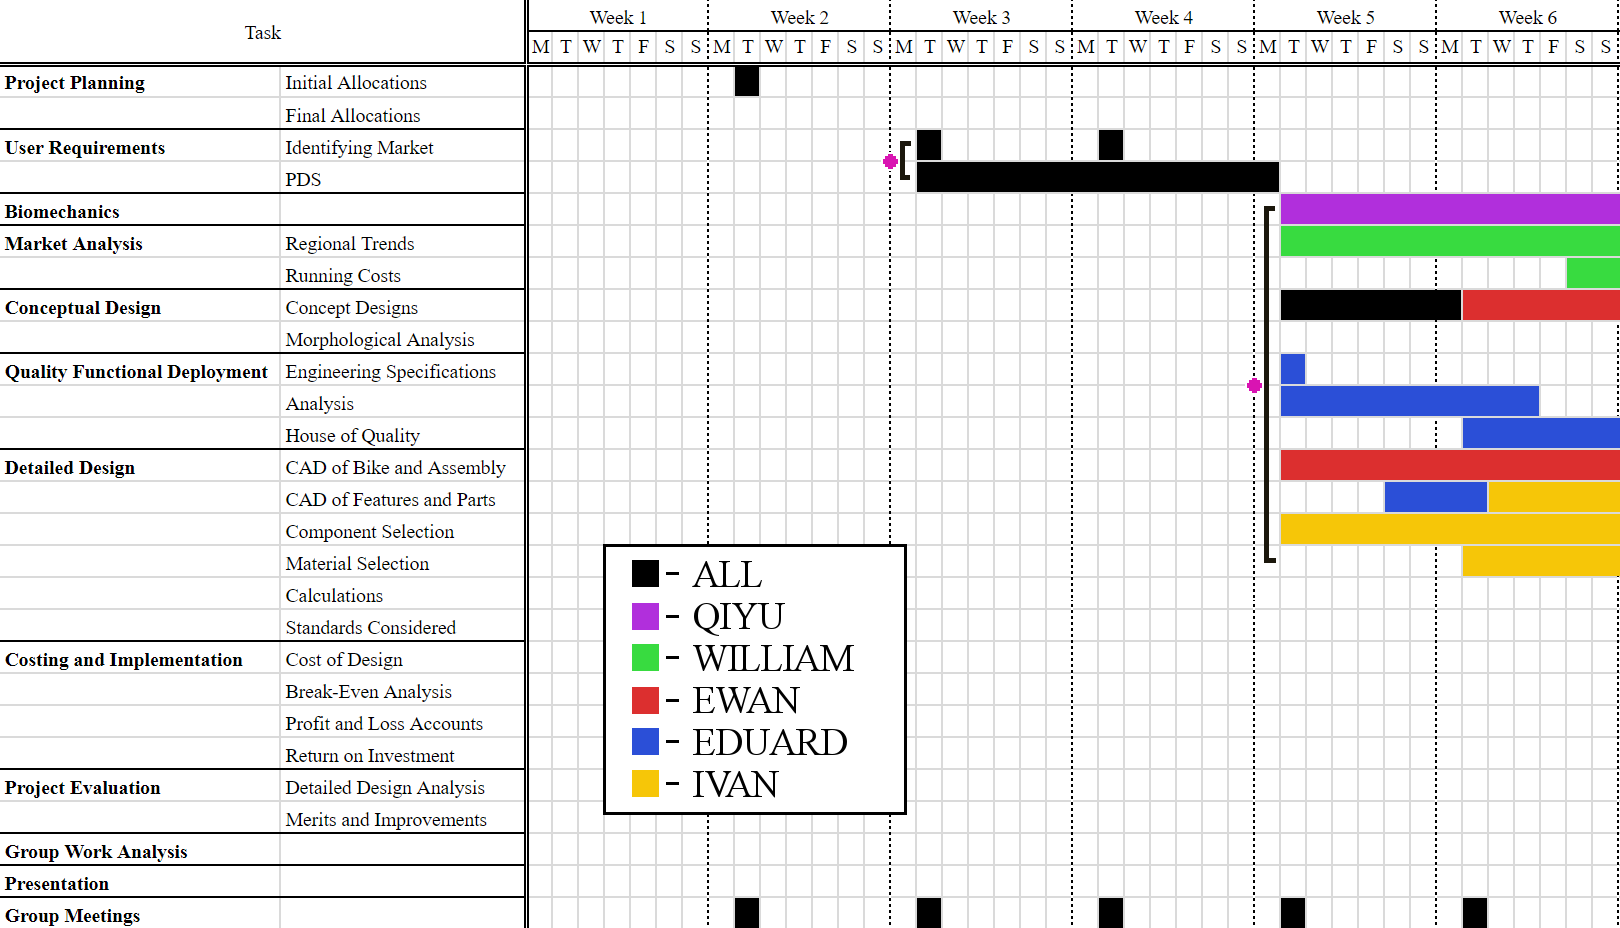
\includegraphics[width=1.44\textwidth]{ganttchart1}
	\label{tab:gtc1}
\end{table}
\vspace*{\fill} 

\newpage

\vspace*{\fill} 
\begin{table}[!ht]
	\centering
	\caption{Gantt Chart Weeks 7-13}
	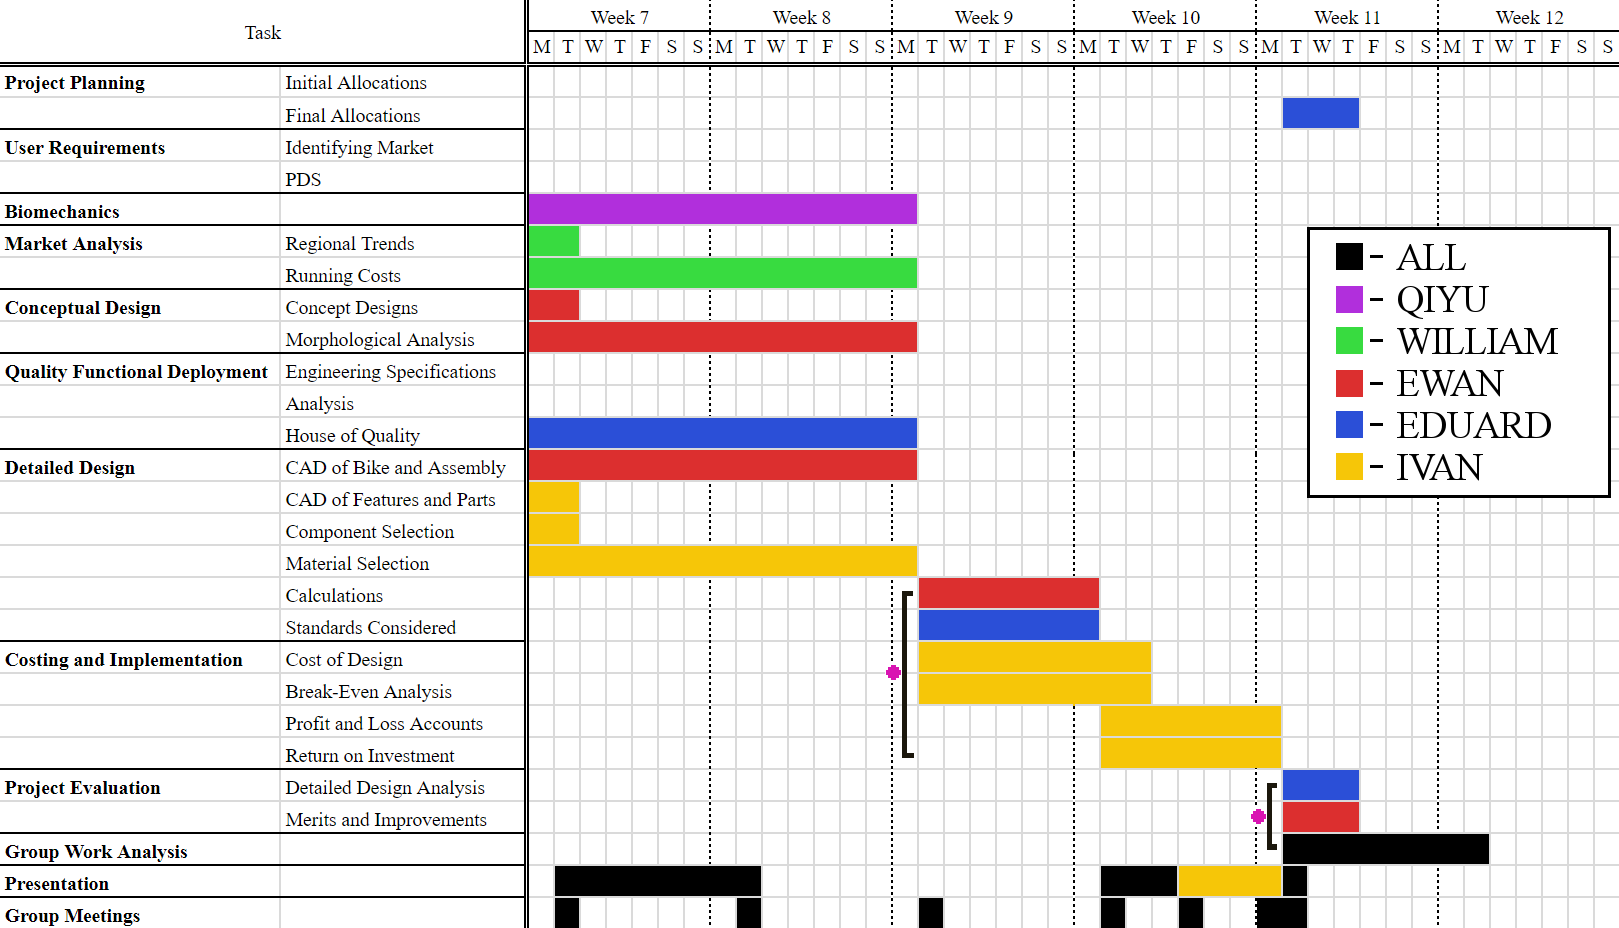
\includegraphics[width=1.44\textwidth]{ganttchart2}
	\label{tab:gtc2}
\end{table}
\vspace*{\fill}
\end{landscape}
\restoregeometry

\section{User Requirements}


\subsection{Identifying the Target Market}

An initial deconstruction of the design brief led to a set of characteristics which would define the project's target market. These are shown below and have been used as guidelines to develop a PDS which focuses on delivering the best solution to the problem at hand.

\begin{itemize}
	\setlength{\itemsep}{0pt}
	\item Designed for a 55+ year old man who is commuting to work in the city
	\item Design should be comfortable and accommodate non-conventional riding gear such as a full suit
	\item Expected to be transporting at least one piece of luggage, e.g. briefcase
	\item Wants to arrive to work without being sweaty
	\item Relatively fit, travelling a maximum of 40 kilometres per day (20 to and 20 back)
	\item Tenured employee with sufficient funds
\end{itemize}

\subsection{Product Design Specification}
\label{sec:pds}

\begingroup
\onehalfspacing
\begin{longtable}{l l c}
	\caption{PDS and Importance scale}\\
	\hline
	Category&Specification&Importance (1-5)\\\hline
	\makecell[l]{Technical Requirements\\ \\}&\makecell[l]{Despite being electrically assisted, operation for \\the user should resemble that of a normal push bike}&\makecell[c]{3}\\ \cline{2-3}
						 &\makecell[l]{According to EU regulations, the motor will assist\\up to maximum speeds of 25 km/h}&\makecell[c]{5}\\ \cline{2-3}
						 &\makecell[l]{The bike's structural integrity should withstand worst\\case loading scenarios without permanent\\deformations}&\makecell[c]{5}\\ \cline{2-3}
						 &\makecell[l]{Mechanical components should withstand at least\\20,000 operational hours}&\makecell[c]{4}\\ \cline{2-3}
						 &\makecell[l]{The frame should withstand the weight of a\\55-year-old man up to the 95\textsuperscript{th} percentile $\approx$ 113kg}&\makecell[c]{4}\\ \cline{2-3}
						 &\makecell[l]{Wheels, rims, gearing, and turning angles should be\\optimised for a city environment}&\makecell[c]{3}\\ \cline{2-3}
						 &\makecell[l]{According to EU regulations, maximum motor power\\of 250W.}&\makecell[c]{5}\\ \cline{2-3}
						 &\makecell[l]{Components should not be compromised structurally\\and accommodate for thermal expansion between -30\\to 60$^{\circ}$C}&\makecell[c]{2}\\ \cline{2-3}
						 &\makecell[l]{Design should accommodate a solution for\\comfortably transporting at least one suitcase.}&\makecell[c]{4}\\ \cline{2-3}
						 &\makecell[l]{Full-cycle recharging of the battery should be within\\4 hours}&\makecell[c]{3}\\ \cline{2-3}
						 &\makecell[l]{Battery should offer a minimum range of 40 km} &4\\ \hline
	Ergonomics&Design should offer a comfortable riding position&4\\ \cline{2-3}
		  &\makecell[l]{Emphasis on comfort should be placed on points of\\contact such as the handlebars and the seat.}&\makecell[c]{3}\\ \cline{2-3}
		  &\makecell[l]{Bike geometry should not stress common points of\\injury such as lower/upper back, neck, and knees.}&\makecell[c]{3}\\ \cline{2-3}
		  &\makecell[l]{A  non-trained person could assemble/disassemble the\\bike within 60 minutes.}&\makecell[c]{2}\\ \cline{2-3}
		  &\makecell[l]{Feet should not slide off the pedals during\\normal operation.}&\makecell[c]{3}\\ \cline{2-3}
		  &\makecell[l]{Battery should be rechargeable from a conventional\\outlet, such as the ones found at home or work.}&\makecell[c]{5}\\ \cline{2-3}
		  &\makecell[l]{Bike should offer different driving modes such as\\disengaging the motor and economy mode.}&\makecell[c]{3}\\ \hline 
	\makecell[l]{Maintenance\\ \\}&\makecell[l]{Battery should not require changing or maintenance\\for at least 1,000 charging cycles.}&\makecell[c]{3}\\ \cline{2-3}
				      &\makecell[l]{Mechanical components which are non-specific for\\the bike design should be readily available}&\makecell[c]{4}\\ \cline{2-3}
				      &\makecell[l]{Motor should be reliable, and in case of failure it\\should be serviced by an expert mechanic}&\makecell[c]{4}\\ \cline{2-3}
				      &\makecell[l]{Sensors and tools available on-board of bicycle, \\should offer the user information about possible\\system failures}&\makecell[c]{2}\\ \cline{2-3}
				      &\makecell[l]{Battery should be easily accessible whilst being\\shielded from the environment}&\makecell[c]{3}\\ \cline{2-3}
				      &\makecell[l]{To avoid mechanical component degradation, mild\\corrosion resistance should be provided for water,\\salt, dust, wind, ice, rocks, oil, and gasoline.}&\makecell[c]{3}\\ \cline{2-3}
		   &\makecell[l]{Suspension should not only provide comfort for the\\user, but also protect the electrical hardware.}&\makecell[c]{4}\\ \hline
	\makecell[l]{Safety\\ \\}&\makecell[l]{A full stop from 25 km/h should be achieved within\\a braking distance of 8 m.}&\makecell[c]{4}\\ \cline{2-3}
				 &\makecell[l]{Chain should be protected from the driver's attire\\and environment}&\makecell[c]{3}\\ \cline{2-3}
				 &\makecell[l]{Street accessories as per law, such as lights,\\reflectors, and brakes.}&\makecell[c]{5}\\ \cline{2-3}
				 &\makecell[l]{Battery should be compatible with different outlets\\and standards to avoid failure during charging.}&\makecell[c]{5}\\ \cline{2-3}
				 &\makecell[l]{Control system should include a feedback loop to\\avoid exposing components to voltages and currents\\outside operational ranges.}&\makecell[c]{5}\\ \cline{2-3}
	      &\makecell[l]{The explosion from a punctured tyre should be\\minimised.}&\makecell[c]{4}\\ \hline
	\makecell[l]{Cost\\ \\ }&\makecell[l]{Final product price should be exactly at the market\\average of \textsterling 1,960 (further discussed in Section~\ref{sec:runc})}&\makecell[c]{4}\\ \cline{2-3}
				  &\makecell[l]{Self-maintenance cost should be similar to that\\of a conventional push bike.}&\makecell[c]{3}\\ \cline{2-3}
				  &\makecell[l]{Battery replacement should be within the range of\\ \textsterling 200 - \textsterling 300.}&\makecell[c]{1}\\ \cline{2-3}
				  &\makecell[l]{Average market price (disregarding economies\\of scale) should be taken for individual components\\and materials for the cost report}&\makecell[c]{3}\\ \cline{2-3}
				  &\makecell[l]{The bike should be a long-term investment with an\\ensured ROI when compared to conventional\\transport methods offered within the city (incentive\\for potential customers)}&\makecell[c]{5}
	\label{tab:pds}
\end{longtable}
\endgroup

The PDS has every specification rated from 1 to 5 in terms of its importance to the final design, with 5 being most important. The majority of the most important points are to do with the standards that must be complied with when designing and selling a bike in Europe. 

The standards that need to be complied with are ones which outline the motor and battery performance of an e-bike \cite{15194}, and another which adheres to general bicycle safety \cite{14764}. The next most important points were generally to do with ease of use for the user, and rider satisfaction. After that came points that should be adhered to naturally as part of designing a bike, and would not require specialised adaptations. The least important aspects were points that are desirable but not required.

\section{Biomechanics}
\label{sec:biomech}

The most attractive part in regards to an e-bike is that it is able to provide assistance in proportion to how much the rider pedals. This allows the rider to conserve energy and reduce their effort while commuting. 

For both e-bikes and ordinary bikes, there are two basic riding mechanics that can be identified in Figure~\ref{fig:peds}. Firstly, the hip flexion which is the extension of hip and knee in positions between 70$^{\circ}$ and 140$^{\circ}$ (see Figure~\ref{fig:knex}), between the quadriceps and calf muscles. Secondly, the knee flexion which is  the extension of muscles in the leg at the bottom and top of the pedal stroke. However, the big difference for an e-bike in comparison to an ordinary push bike, is that the quadriceps and gluteus muscles will require less force to bring one pedal to the top position. Additionally, less downward force will be required by the hamstring and calf muscles to the opposite pedal.

\begin{figure}[!ht]
\centering
	\begin{minipage}{.5\textwidth}
		  \centering
		  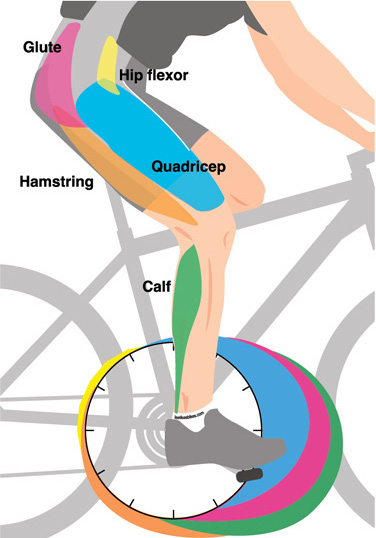
\includegraphics[width=.4\linewidth]{peds}
		  \captionof{figure}{Muscles Involved in pedal stroke}
		  \label{fig:peds}
		  \cite{lee08}
	\end{minipage}%
	\begin{minipage}{.5\textwidth}
		  \centering
		  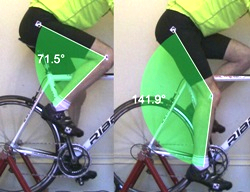
\includegraphics[width=.75\linewidth]{knex}
		  \captionof{figure}{Hip flexions and the relative position}
		  \label{fig:knex}
		  \cite{bd16}
	\end{minipage}
\end{figure}

The main cause for the big difference in force required, comes from the propulsion provided by the pedal motor. This propulsion is applied to the rear wheel, and is the main motivation of the final design. A conventional electric motor on a bicycle, is able to assist the rider by up to 250\% (complying to the EU legal standard). Thus allowing the rider to save up to 70\% of the force and effort required on an ordinary push bike in comparison \cite{bosch18}.

In terms of the upper part of the human body, the same muscles are engaged regardless of the type of bike. This comprises of the abdominal muscle, which is responsible for the cycler's spine, and ensuring balance, in the pelvis and spine. Moreover the muscles in the upper and lower arms allow the rider to grip the handlebars. 

Due to the already low effort required by the lower part of the body, the design of the frame was prioritised to give the user a comfortable riding position. Following the guidelines established in the PDS, it was determined that an up-right riding position, where the spine is straight would lead to: a decrease in force required by the abdominal and arm muscles to hold the riding posture. This will contribute to less stress in the back, spine, and neck of the rider \cite{schwell05}.  

\section{Current Market Analysis}
\label{sec:CAA}

E-bikes have been, and are, continuing to be the highest selling electrical assisted vehicle on the planet, with nearly 35 million unit sales forecast in 2016 \cite{citron16}. Many factors are behind this reason of high-sales such as: its lower cost relative to cars, no licensing requirements from the user, and improvements in their technologies, mainly in the Lithium ion, or Li-ion battery, making it cheaper and lighter. This demonstrates the unique position that e-bikes are exposed to, to become a primary benefactor of this trend.

\subsection{Regional Trends}

Within the regional trends, the global e-bike markets are well-positioned towards huge growths, primarily within the Li-ion battery section. Although sealed lead-acid (SLA) batteries continue to represent the largest segment of e-bikes due to lower costs and popularity in China, the market share of this type of battery will decrease significantly over the next few years, because of the bad environmental impacts and the increasing performance of Li-ion batteries \cite{wood17}. E-bike industries are driven from the high urbanisation rates, improvements in technologies of batteries and bicycling infrastructure, aggressive energy rules and policies, low cost and many others. However, the low costs in gasoline, low consumer awareness, and high costs relatively to traditional bicycles have impacted restricting sales in some markets.

The Asia-Pacific excluding Japan (APEJ) region, is expected to lead the global e-bike sales industry. However in China, the world's largest market within the annual sales of the e-bikes using SLA batteries, are expected to have their sales decline because of the market saturation and laws, regarding bans on e-bike usage in large areas of major cities including: Beijing, Shanghai, etc. However, sales of Li-ion e-bikes will grow significantly over the forecast period, due to the strong support from the government towards the technology. Thus, the APEJ region is expected to lead the global e-bike sales industry \cite{citron16}.

On the other side of the world, Western Europe continues to achieve a steady significant growth in the e-bike industries, with Germany alone having 535,000 unit sales in 2015, from 480,000 in 2014 \cite{citron16}. According to Navigant Research, the e-bike sales are expected to naturally replace bicycle purchases in Western Europe.

In North America, the e-bike market remained relatively flat in 2015, because of the low retail gasoline prices. Nevertheless, the United States still has huge potential for e-bikes due to its extensive bicycle market, which accounts for roughly 16 million sales per year \cite{citron16}.

Overall, the global e-bike market is projected to grow at 0.4\% compound annual growth rate, or CAGR, within the forecast period from 2016 until 2025. Compound annual growth rate is used to measure the market growth over multiple time periods. The slow growing CAGR is largely due to China's anticipated decline in annual unit sales, stated previously, at -0.8\% CAGR. Excluding China however, the CAGR growth will be around 8.2\% \cite{citron16}. This demonstrates an expected strong growth in the market, in which annual unit sales will rise from 3.3 million in 2016, to nearly 6.8 million units by 2025. This growth is expected to occur mostly in Western Europe and within Asia Pacific, including Japan. The graphs below (Figure~\ref{fig:crw}, Figure~\ref{fig:inve}) shows the annual e-bike sales of different regions within the period of 2016 until 2025.

\begin{figure}[!ht]
	\centering
	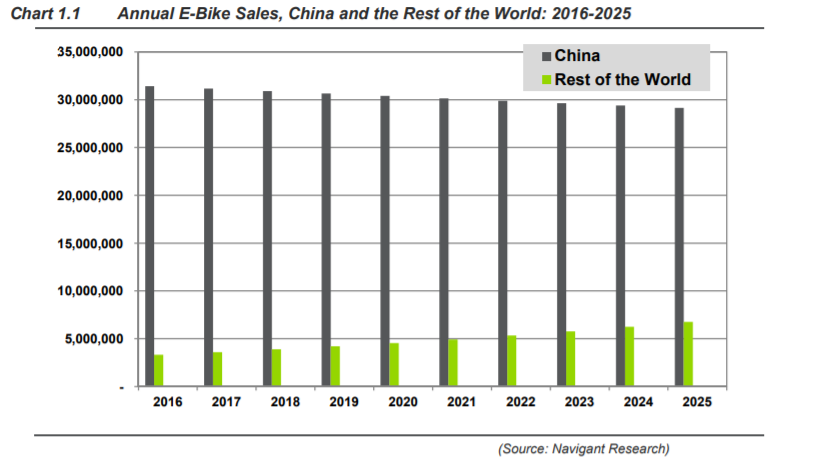
\includegraphics[width=0.85\textwidth]{ebsale}
	\caption{Annual e-bike sales, China and the rest of the world}
	\cite{citron16}
	\label{fig:crw}
\end{figure}

\begin{figure}[!ht]
	\centering
	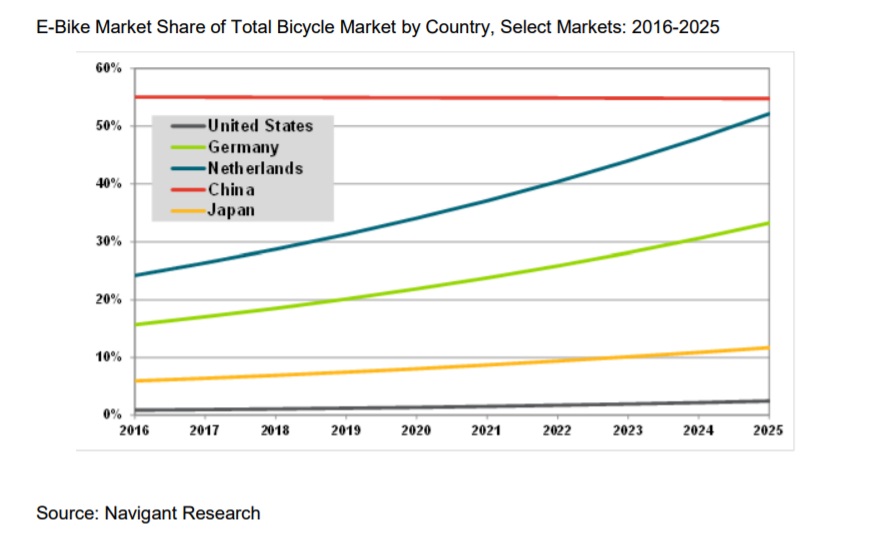
\includegraphics[width=0.85\textwidth]{ebmarketshare}
	\caption{E-bike market share of total bicycle market by country}
	\cite{citron16}
	\label{fig:inve}
\end{figure}

\newpage

\subsection{Running Costs}
\label{sec:runc}

The global e-bikes market research report has profiled many key companies in the market. Companies such as Robert Bosch GmbH, Panasonic Corp, Samsung SDI Co., Ltd., and many others are keenly interested in increasing their investments toward e-bikes. The list below depicts some of the few companies already involved within the e-bike industry.

\vspace{2em} 
\begin{minipage}[l]{0.45\textwidth}
\begin{itemize}
	\setlength{\itemsep}{0pt}
	\item Robert Bosch GmbH
	\item Accell Group N.V.
	\item Giant Manufacturing Co., Ltd.
	\item Derby Cycle Holding GmbH
	\item Jiangsu Xinri E-Vehicle Co. Ltd
	\end{itemize}
\end{minipage}
\begin{minipage}[r]{0.45\textwidth}
	\begin{itemize}
	\setlength{\itemsep}{0pt}
	\item Panasonic Corp.
	\item Bionx International Corporation
	\item Mahindra \& Mahindra Ltd.
	\item Samsung SDI Co., Ltd.
	\item Prodeco Technologies Llc
\end{itemize}
\end{minipage}
\vspace{2em} 

Inspecting the listed companies, the costs of different types of e-bikes can be summarised:

\begin{table}[!ht]
	\centering
	\caption{Type of E-Bike and the allocated retail price}
	\begin{tabular}{l r r}
		\hline
		Type of E-Bike&\makecell[l]{Average Cost (\$)}&\makecell[l]{Range (\$)}\\ \hline
		Cruiser Bicycle	&3050	&1500 -- 7900\\
		Mountain Bicycle	&4150	&1200 -- 9000\\
		Road Bicycle	&4750	&1900 -- 8000\\
		City Bicycle	&2800	&1200 -- 8000\\
		Folding Bicycle	&1750	&700 -- 5000\\
		Cargo Bicycle	&3300	&1700 -- 6000\\
	\end{tabular}
	\label{tab:pri}
\end{table}

\subsection{Conclusion}
\label{sec:caac}

Following the information obtained in the market analysis, a series of further conclusions were made with regards to the project's specific design. 

First, it was decided that Li-ion batteries would be used due to their technical advantage and future potential for development. Furthermore, the analysis of regional trends has shown that within the EU (market for which this bike is being specifically designed), the greatest market share (by far) belongs to the Netherlands and Germany (see Figure~\ref{fig:inve}). Therefore, a design tailored towards these locations would be beneficial in establishing the company within its developed market. The design would encompass a more classical looking bike which would integrate into the business environment, as opposed to the sport-like e-bikes that the market is currently saturated with. 

Finally, it was decided that the target price would be the average in the city e-bike category. As seen in Table~\ref{tab:pri}, this is equivalent to \$2,800. Using the current conversion rate (\$1 = \textsterling 0.70), the final target price is obtained to be: \textsterling 1,960.00 \cite{xe}.

\section{Conceptual Design}

\subsection{Concept Sketches}

The following are concept sketches (Figure~\ref{fig:sk}) which correspond to ideas 1-5, in order, in the subsequent morphological analysis. The second sketch has been rendered by hand to show the colour scheme that has been approved by the group. The chosen black/grey colour scheme is utilised as it gives a classy and mature look, and would best appeal to the specified target market of more classy and mature men. The sketches, morphological analysis, in conjunction with the most popular choices from it, conceptualised the final design choice, Figure~\ref{fig:fs}. 

The sketches allowed for a better understanding of how the design might be implemented, and how to construct it as visually appealing. This plays a major part of any design in terms of marketing and sales. 

\begin{figure}[!ht]
	\centering
	\includegraphics[width=0.98\textwidth]{ske}
	\caption{First concepts}
	\label{fig:sk}
\end{figure}

\begin{figure}[!ht]
	\centering
	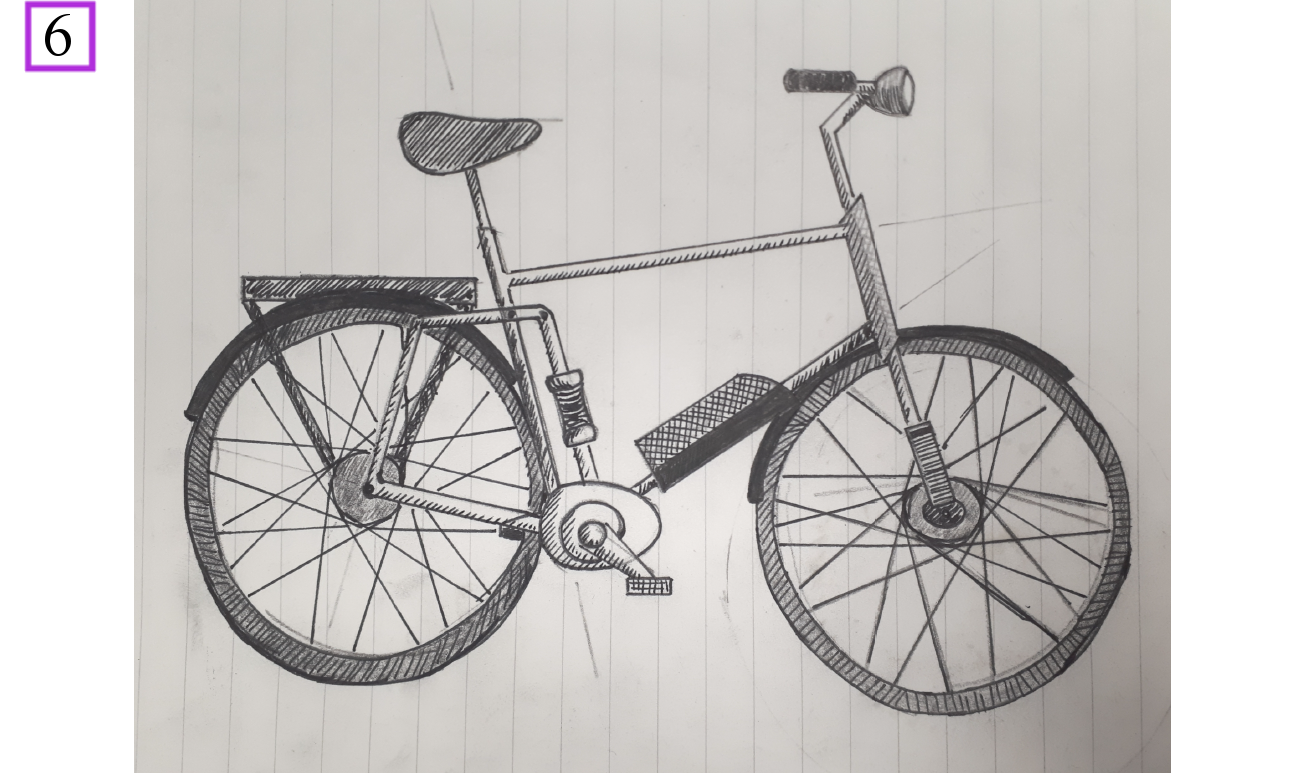
\includegraphics[width=0.7\textwidth]{fic}
	\caption{Final concept}
	\label{fig:fs}
\end{figure}

\subsection{Morphological Analysis}

\begin{table}[!ht]
	\centering
	\caption{Morphological analysis with 6 designs. For colours refer to Figures~\ref{fig:sk} and~\ref{fig:fs}}
	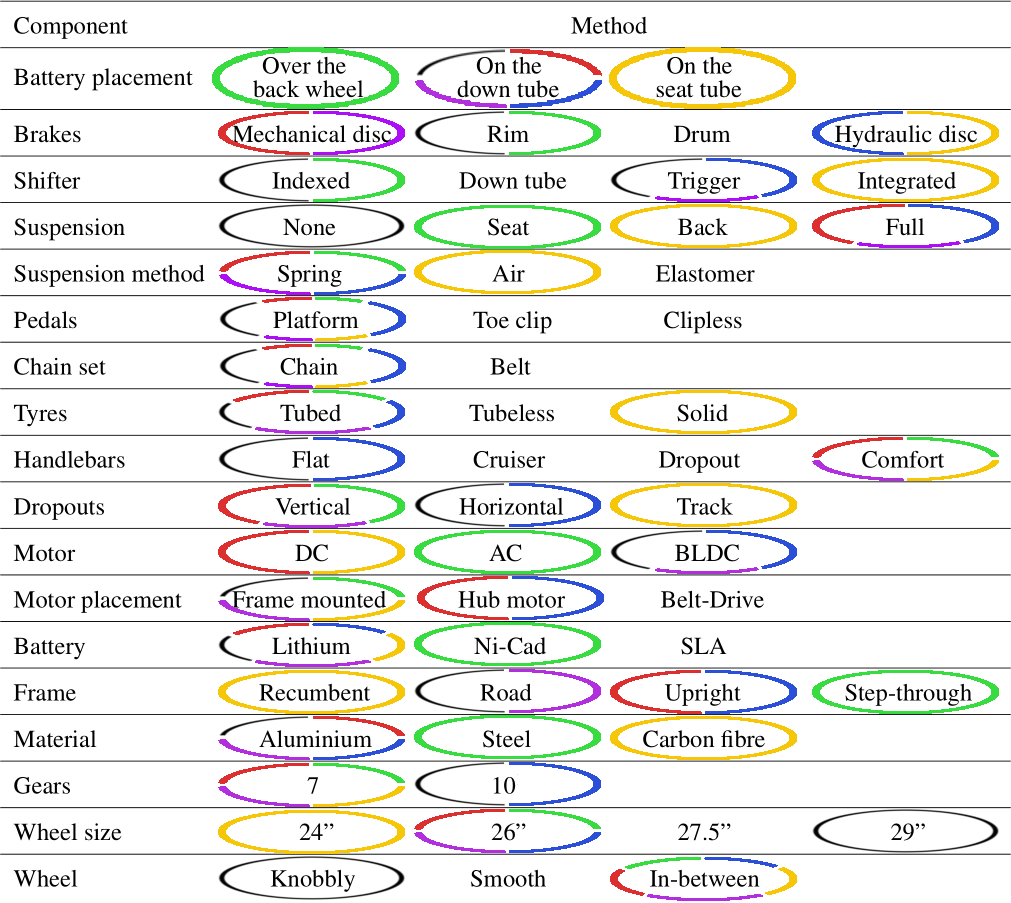
\includegraphics[width=0.98\textwidth]{morph}
\end{table}

The following points explain how each method is considered when choosing the correct component for the final design.

\begin{enumerate}[leftmargin=0pt, itemindent=20pt,labelwidth=15pt, labelsep=5pt, listparindent=0.7cm,align=left]
	\item Battery Placement:

Identified based on different placements, as the battery can affect the centre of gravity of the bike and therefore its steering. This can cause possible grievances to the user due to difficulty in handling with the battery, and can also get in the way of other possible features to the bike such as a luggage rack.

	\item Brakes:

Decided on based on the relative price, braking power, and ease of maintenance. Rim brakes are the cheapest, while disc brakes have the most braking power. Furthermore, mechanical mechanisms are cheaper than hydraulic mechanisms, and drum brakes are the least common.

	\item Shifter:

Determined in terms of ease of use and price, with trigger being the easiest shifters to use but being on the more expensive side compared to indeed or integrated. Down tube shifters are considered the most difficult to use.

	\item Suspension:

More suspension provides a better ride but is more expensive. However, full suspension is considered the best option based on the primary objective.

	\item Suspension method:

Criticised in terms of price as the differences in their abilities is relatively negligible for the purpose of a city bike. Spring suspension is considered the cheapest method.

	\item Pedals:

Considered briefly, and it was determined that only the simplest method coincided with the objective.

	\item Chain set:

Considered briefly, as using a chain instead of a belt is the best choice by far. This is due better efficiency for the high torque capabilities of an e-bike.

	\item Tyres:

Observed in terms of the amount of tread, and the type of tubing of the tyres. The tread was inspected with regard to safety vs. ease of use, with the more treaded tyres being safer but also harder to utilise due to the increase in friction. The tubing types were looked at in terms of ease of use/maintenance with tubed being the best.

	\item Handlebars:

Examined in terms of ease of use, with comfort being an important factor as well as usability.

	\item Dropouts:

Inspected in terms of ease of use/maintenance, with vertical being the easiest to use, but horizontal adding to the adjustability of a design.

	\item Motor \& Placement:

The motor type was investigated in terms of performance vs. price, with BLDC providing the best performance at the most expensive price. The motor position was looked at in terms of performance, with hub motors affecting the centre of gravity the least.

	\item Battery:

		Considered in terms of performance vs. maintenance, with lithium-ion being the currently emerging battery type (see Section~\ref{sec:CAA}). 

	\item Frame:

Examined in terms of aesthetic appeal, and usability. Road and upright frames were concluded as being better for the back, and appeals better to the target audience.

	\item Material:

Identified based on price vs. performance with aluminium being the cheapest, carbon fibre being the best performing, and steel being a good middle ground.
	
	\item Gears:

Analysed in terms of price vs. performance with less gears being cheaper but allowing less options when riding.

	\item Wheels \& Size:

The wheel size was looked at in terms of performance vs. maintenance, with 26'' being the most common wheel size. The In-between tyre grants a combination between pedal efficiency and grip, which allows for adequate use in typical weather conditions.

\end{enumerate}

\subsection{Conclusion}

From the 5 different ideas that were evaluated in the morphological analysis, the final concept (Figure~\ref{fig:fs}) was created by choosing the most popular method illustrated, whilst ensuring that all the choices made work together and reinforce each other. 

Firstly, it was decided to adopt the aesthetics of concepts 1 and 2 into the final design (refer to Figure~\ref{fig:sk}). Every concept used platform pedals as these are the easiest to use and don't require any special equipment, thus they are more likely to be desirable to the target market. All concepts used a chain rather than a belt as a chain-set, due to its durability and ease of replacement. Almost all of the ideas used lithium ion batteries as these are the most commonly found batteries and are consistently becoming more powerful. Furthermore, nearly all of the designs are made from aluminium, as it is a fairly cheap material with good stress and strain capabilities, whilst also being relatively lightweight. Finally, the use of full suspension allows: a decrease in heart rate by 20-50 beats/min, oxygen requirement by 30\%, and 30-60\% less required power to maintain the same speed by the rider \cite{glaskin12}. This perfectly accommodates the concerns addressed in the design brief, and is therefore utilised.  

The final concept thus includes the following methods:

\begingroup
\onehalfspacing
\begin{longtable}{l l}
	\caption{Final concept selected method and reasoning}\\
		\hline
		Component&Method and Reasoning\\\hline
		Brakes&\textbf{Mechanical disc brakes} are used due to their better braking power.\\
		Shifter&\textbf{Trigger shifters} for convenient gear changes.\\
		Suspension&\textbf{Spring suspension}, as it is a cheaper method of suspension than compressed air.\\
			  &\textbf{Full suspension} because of the weight of an e-bike, and its electrical components.\\ 
		Pedals&\textbf{Platform pedals}, as they require no specialised equipment.\\
		Drive train&\textbf{Chain} rather than belt, due to better durability and replacement options.\\ 
		Dropouts&\textbf{Vertical}, for ease of use and quick wheel replacements.\\
		Motor&\textbf{BLDC}, due to its reliability over the other options.\\
		     &\textbf{Frame-mounted motor}, due to simplicity in terms of maintenance and for affecting\\
		     &\phantom{WW} the centre of gravity the least.\\ 
		Battery&\textbf{Lithium-ion}, most commonly used batteries that are reliable, and easy to replace.\\
		       &Placed on the \textbf{down tube}, keeps the battery out of the way of the rider and \\
		       &\phantom{WW} distributes its weight the most naturally.\\
		Frame&Resemble a city bike but with elements of a more \textbf{upright bike frame} to it, this is to\\
		     &\phantom{WW} try and appeal to the target market with a more stylish frame compared to\\
		     &\phantom{WW} the usual bulky e-bikes on the market.\\
		Material&\textbf{Aluminium}, as it is relatively light, cheap and strong. \\
		Gears&Standard \textbf{7 gear configuration}, as it is the most appropriate for a city environment.\\ 
		Wheel size&Standard \textbf{26''}, give the bike the easiest/most comfortable ride.\\
		Tyres&Not overly treaded but will also not be bald like road bike tyres, it will be \textbf{in-between}\\
		     &\phantom{WW} such that the tread will provide sufficient grip during wet weather, but will \\
		     &\phantom{WW} not make it hard to pedal during dry weather.\\
		     &\textbf{Tubed tyres} will be used as they are easy to maintain.\\
		Handlebars&\textbf{Comfort handlebars} will provide the most relaxed ride. 
\end{longtable}
\endgroup

\section{Quality Function Deployment}

In order to meet customer demands, research and initial product specifications are combined to form the House of Quality. The aim is to produce a customer driven product which will fulfil key demands, by translating user requirements into engineering requirements. Then, by comparing the individual aspects, the importance can be visualised and securely compromised if deemed unimportant to the design \cite{fran01}.

\subsection{Engineering Specifications}

\begin{table}[!ht]
	\centering
	\caption{Translation of user requirements}
	\begin{tabular}{l l l}
		\hline
		Category&User Requirements&Engineering Specifications\\\hline
	Performance&Bike parts will last for a long time&Fatigue Limit Cycles\\
		   &Gearing fit for a city environment&Number of Gears\\
		&Mobility at cruising speeds&Turning radius at moderate speed 15km/h\\
		&Protected against drastic temperatures&Melting point of Material\\
		&Corrosion resistant&Based on material selection\\
		&Luggage space&Amount of suitcases supported\\
		&High acceleration from rest&Effort required for acceleration\\
		&Low-effort for commute&Effort required for distance\\
		&Supports the weight of the rider&Material yield strength\\
		&Good braking&Braking distance from max speed\\
		&Stability at higher speeds&Height of motor above ground\\\hline
	Battery&High battery capacity/battery lifespan&Battery capacity\\
		&Electrical assist speed limit&Output choke speed\\
		&Battery recharges quickly&Recharge cycle time (full)\\
		&Supported power output of the battery&Work output by battery\\\hline
	Suspension&No deformations due to vibrations&Material yield strength\\
		&Good shock absorption&Vibration frequency on rough terrain\\
		&Smooth ride&Adjusted spring stiffness\\\hline
	Ergonomics&Comfortable riding position&Amount of satisfied people\\
		  &Height adjustable seat and handlebars&Range of adjustment (seat)\\
		&Easy to assemble&Assembly time\\
		&Easy to maintain&Amount of tools required\\
		&Easy to carry&Overall weight of bicycle\\
	\end{tabular}
\end{table}

From the product design specifications, specifications from Table~\ref{tab:pds} were grouped together to form an umbrella statement that a potential user might inquire about the bike. For example, ``Mechanical components should withstand at least 20,000 operational hours,'' and ``Motor should be reliable, and in case of failure it should be serviced by an expert mechanic,'' are translated into ``Bike parts will last for a long time.'' 

Some statements from Table~\ref{tab:pds}, were ruled out as they seemed inappropriate towards the objective of the House of Quality. For example, ``The explosion from a punctured tyre should be minimised.'' As well as, the entire category specifying ``Cost,'' was not included as it is essentially how the outcome of the House of Quality is quantified.

When translating user requirements to engineering specifications, various methods of testing and measuring were considered in the process. In terms of performance, properties of the general structure of the bike, and its functionality are considered. Furthermore for the battery and the suspension, characteristics were considered outside of the performance, as they are aspects that must be well defined for the end design of the bike. Lastly, requirements categorised as ergonomics, are quantified in terms of ease of use and comfort.

\subsection{Analysis}

To form the House of Quality, the following investigations were made to find relationships between the requirements:
\begin{itemize}
	\setlength{\itemsep}{0pt}
	\item What vs. How? (User requirements vs. Engineering specifications)
	\item How vs. How? (Engineering specifications vs. Engineering specifications)
	\item Who vs. What? (Potential buyers vs. User requirements)
	\item Now vs. What? (Similar products on the market vs. User requirements)
	\item How much? (What are the feasible targets in terms of engineering specifications)
\end{itemize}

In the first phase of analysis, User requirements and Engineering specifications are inspected for relationships (middle area of Table~\ref{tab:hoq}). First, each engineering specification was identified with its corresponding unit of measurement and the direction in which it should be improved. Furthermore, from the colours it is apparent that the diagonal line of strong relationship is due to each user requirement having its own engineering specification. From this the main points of focus became:
\begin{itemize}
	\setlength{\itemsep}{0pt}
	\item High battery quality as each battery specification compliments each other, and will clearly demonstrate high performance to the user
	\item The weight of the bicycle has a large impact on all other requirements, which means that it must be reduced as much as possible
	\item Suspension, overall comfort, and battery power will be able to reduce the effort of the rider which has a direct correlation with the main objective
\end{itemize}

Next, engineering specifications are evaluated for potential relationships with each other in the roof (Table~\ref{tab:roof}). This analysis further reveals the importance of reducing the weight, and confirms how the effort of the rider will be minimised. The latter requirement primarily requests for sufficient battery quality, which will have to be implemented into the final design. Lastly in terms of suspension, the safety of the rider will essentially be improved, by protecting the bike during operation and potentially reducing braking distances.

Potential buyers are then considered and scored based on how important they find the functional (user) requirements (left columns of Table~\ref{tab:hoq}). In this case, 3 potential buyers are considered, and how they would potentially rank the importance of the selected requirements. The numbers sum up to 100, which means that an average importance lies at around 4 points. The following describes how the scores were evaluated:
\begin{itemize}
	\setlength{\itemsep}{0pt}
	\item The target commuter will value high performance, battery quality, and comfort; in order to maintain expectations over regular use
	\item The recreational user will value battery quality and ergonomics; to uphold the condition over infrequent use
	\item The retailer/sales person will require a balanced bike, with good adjustability to market to a range of customers
\end{itemize}

In order to visualise where the final product would rank within the current market, competitors are scored based on how well they fulfil the same user requirements (right column of Table~\ref{tab:hoq}). Here, a cheap, low-end bicycle (Greenedge CS2) and a high-end, expensive bicycle (Trek Lift+ Men) are qualitatively judged, where 5 is excellent and a 1 is poor (bicycles depicted in Figure~\ref{fig:bcom}). 

The selected design is supposed to fill the price range between the two (see PDS), therefore its ranking is also kept between them. This resulted in a qualitative analysis that concluded: slight improvements in terms of mobility, luggage, and ride quality over the high-end bicycle. These attributes are desired in order to better fulfil the main objective, and tailors the detailed design towards a working man. However, compromises will have to be made appropriately in order to fit the budget (i.e. in other selected categories or in the manufacturing process).

\begin{figure}[!ht]
	\centering
	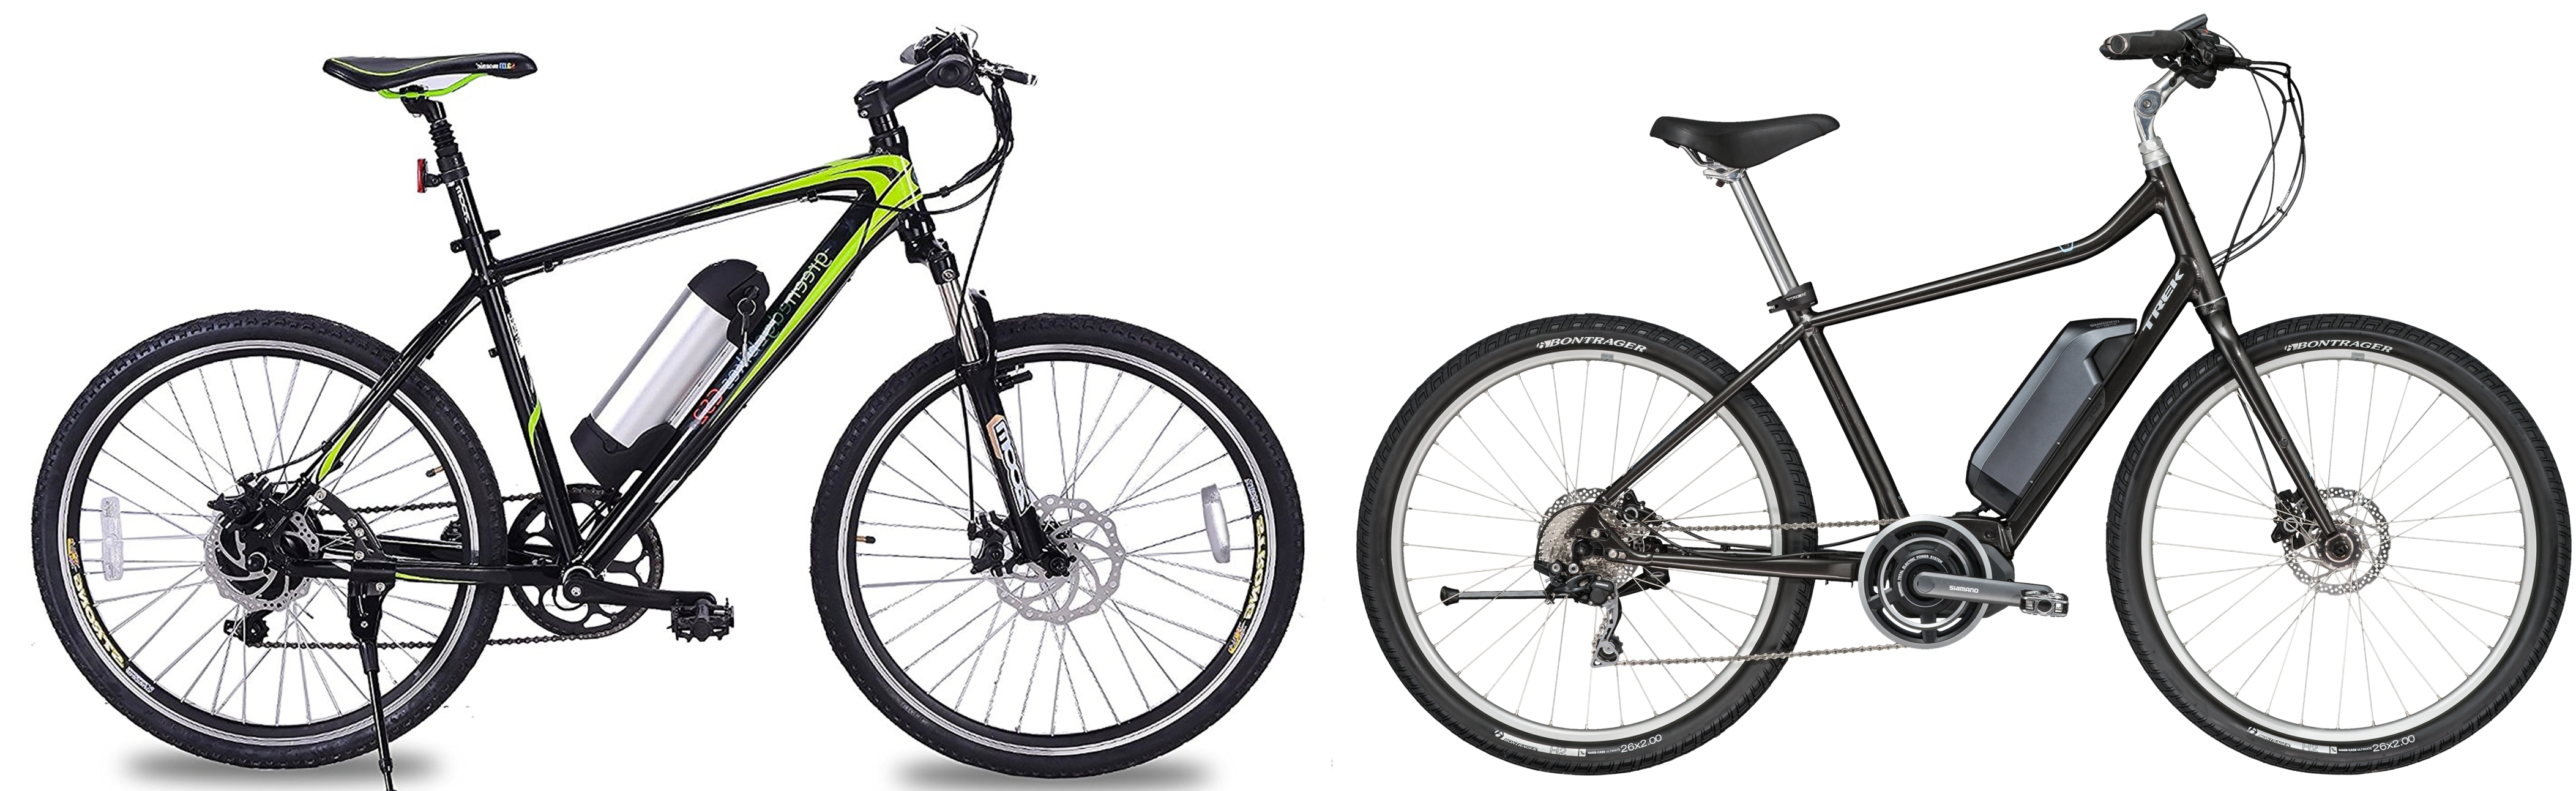
\includegraphics[width=0.98\textwidth]{bikec}
	\caption{Greenedge CS2 (left) priced at \textsterling 869.99  (Halfords, 2018), Trek Lift+ Men's (right) priced at \textsterling 2,299.99 (Trek Bicycle Corporation, 2018)}
	\label{fig:bcom}
\end{figure}

Taking the existing information of the competitors into account, and adjusting to the qualitative rankings, the targets for the design can be specified in the bottom rows of Table~\ref{tab:hoq}. In the case where all values between bicycles are the same, the target was deemed as important, and had to be implemented in the design. Otherwise, a range was given that would correspond to the design's ranking.

As a low-end bicycle for a low price, the Greenedge CS2 bears the worst specifications \cite{cs2}. It's achievements are taken as a baseline that are going to ideally be outperformed by the final design. As a high-end bicycle, the Trek Lift+ Men's sets an upper limit \cite{trek} which would ideally be matched by the final design. Therefore, the final targets almost exclusively outperform the Greenedge CS2, and a delighted target that slightly exceeds the Trek Lift+ Men's ensures room for improvement. In the case where no information was available, preliminary calculations and conventional specifications are indicated in order to specify a sensible target.

\newpage

\newgeometry{margin=0.8cm}
\thispagestyle{empty}
\begin{landscape}

\vspace*{\fill} 
\begin{table}[!ht]
	\centering
	\caption{House of Quality}
	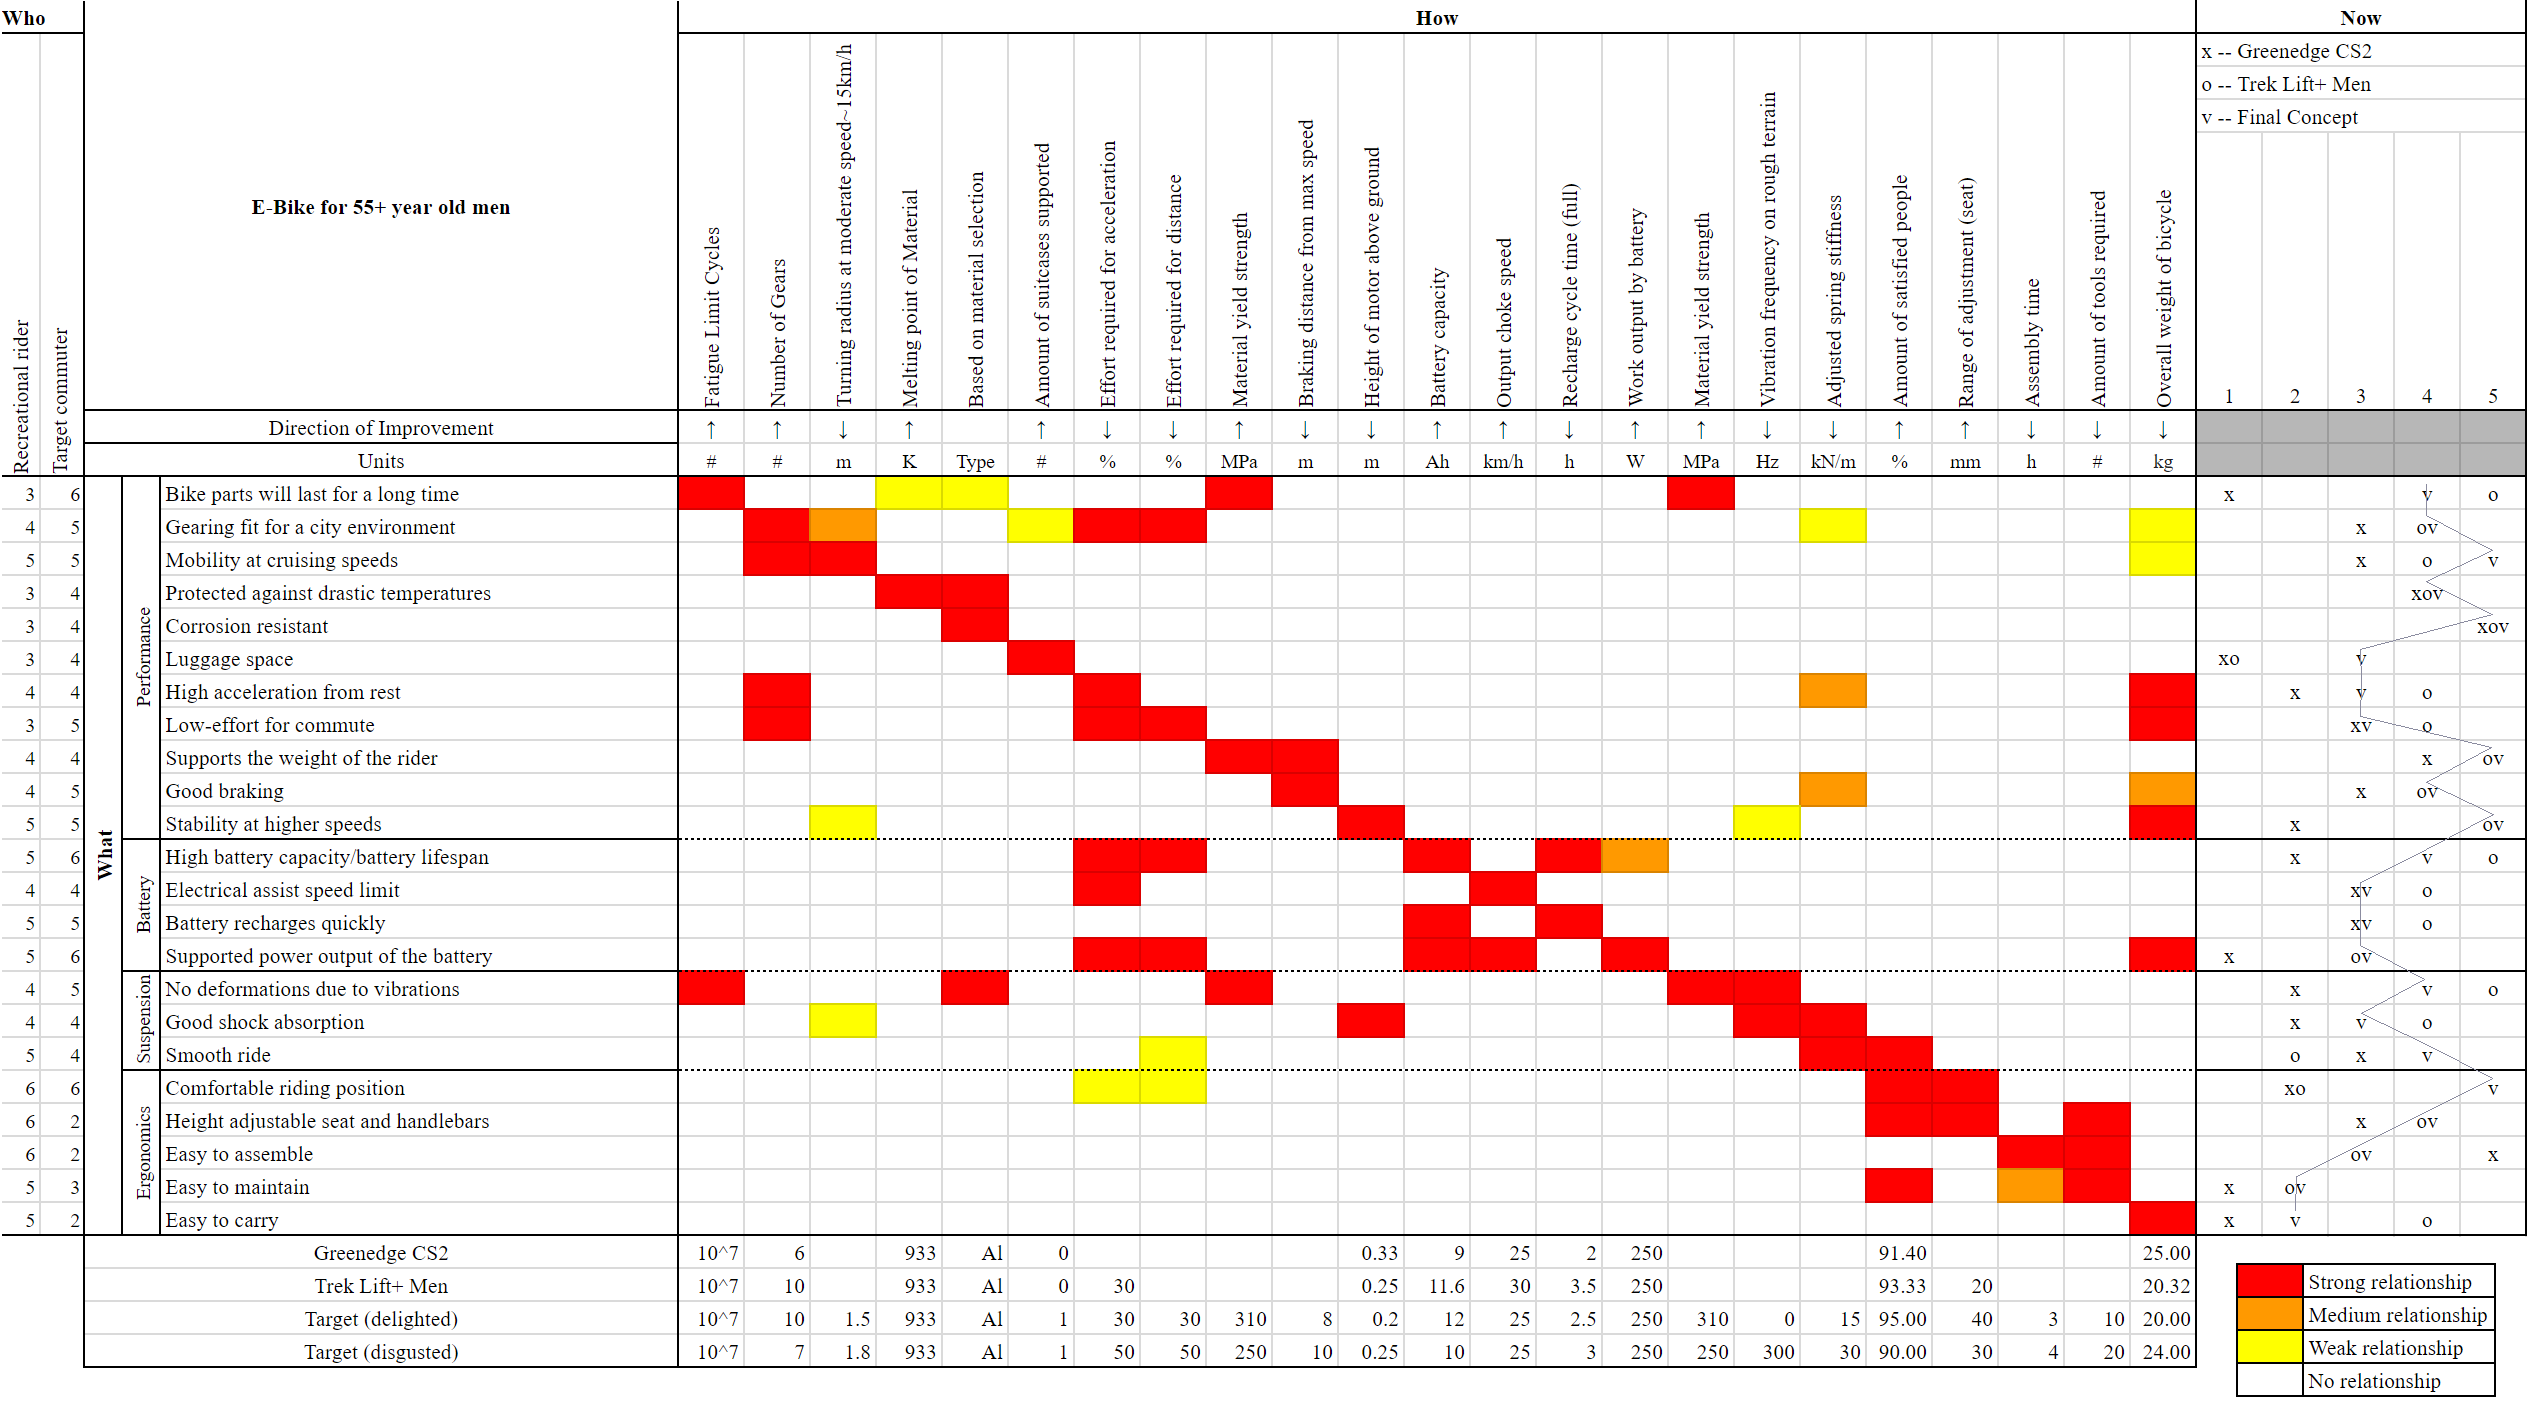
\includegraphics[width=1.44\textwidth]{Hous}
	\label{tab:hoq}
\end{table}
\vspace*{\fill} 

\newpage
\thispagestyle{empty}

\begin{table}[!ht]
	\centering
	\caption{House of Quality roof}
	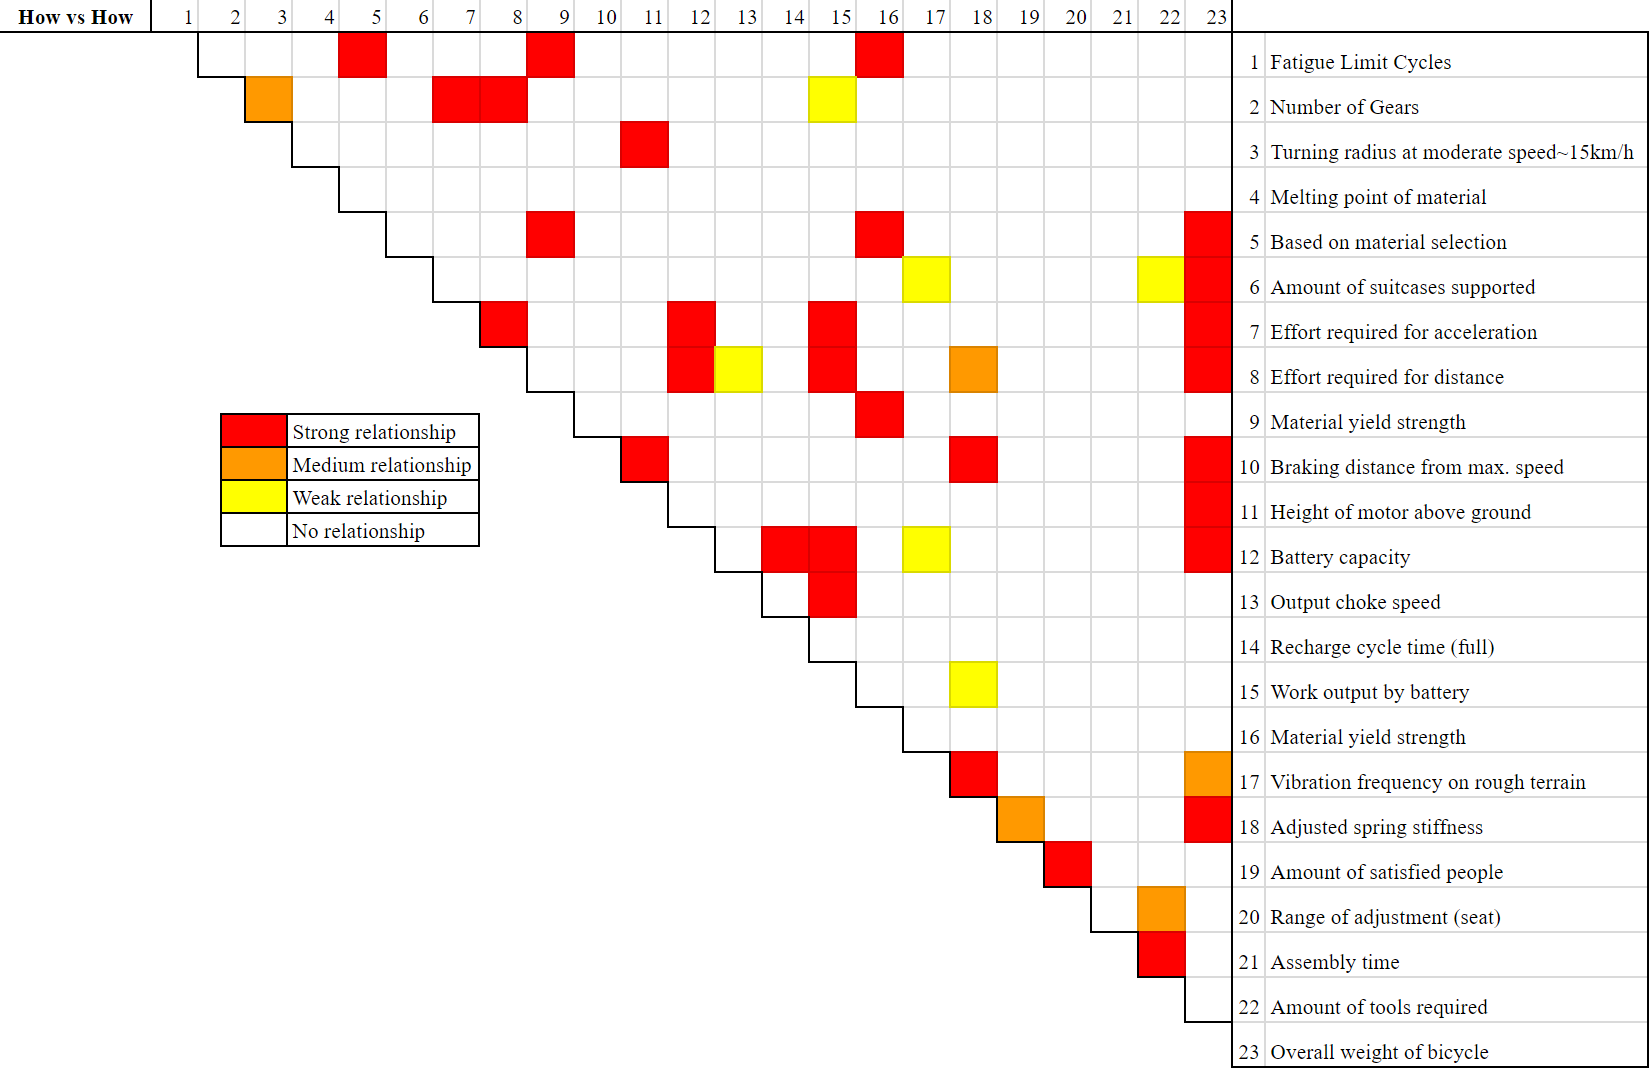
\includegraphics[width=1.44\textwidth]{Roof}
	\label{tab:roof}
\end{table}

\end{landscape}
\restoregeometry

\section{Detailed Design}

\begin{figure}[!ht]
	\centering
	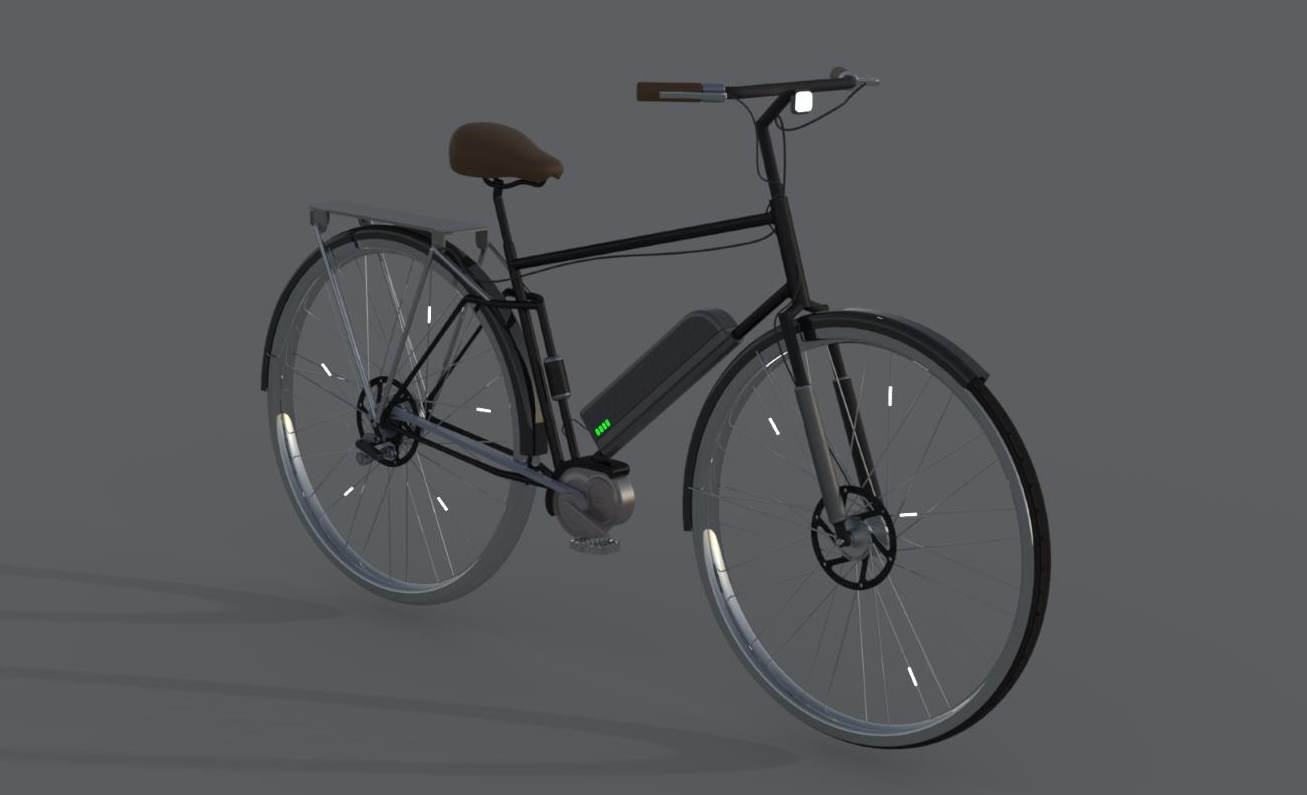
\includegraphics[width=0.98\textwidth]{bikeren}
	\caption{Final Bike render in SolidWorks}
\end{figure}

\begin{figure}[!ht]
	\centering
	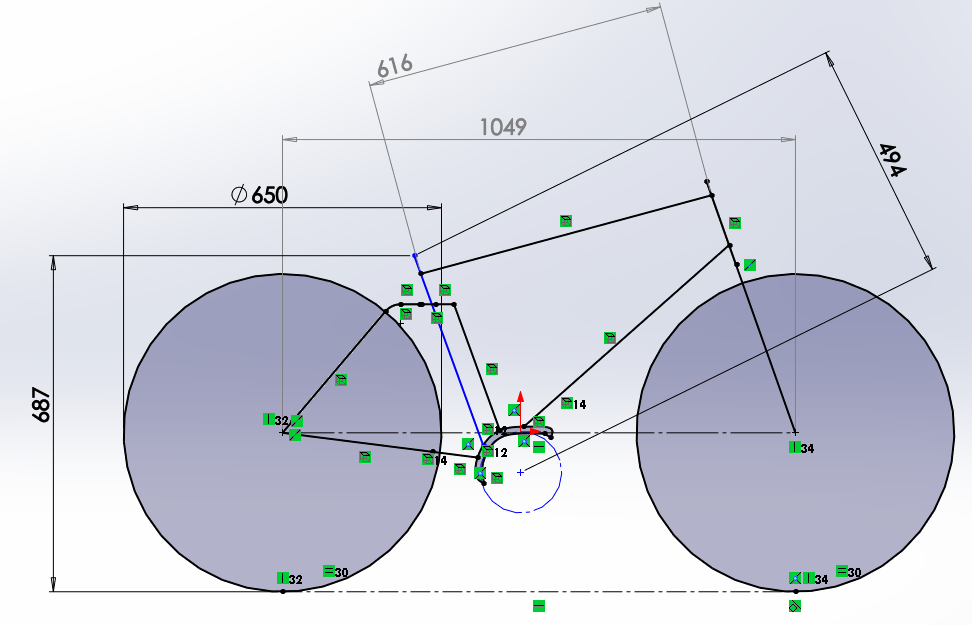
\includegraphics[width=0.98\textwidth]{bikedim}
	\caption{Basic sizings of the bike frame including: wheel size, minimum seat height, centre to centre distance, top tube and wheel centre to centre distance.}
\end{figure}

\begin{figure}[!ht]
	\centering
	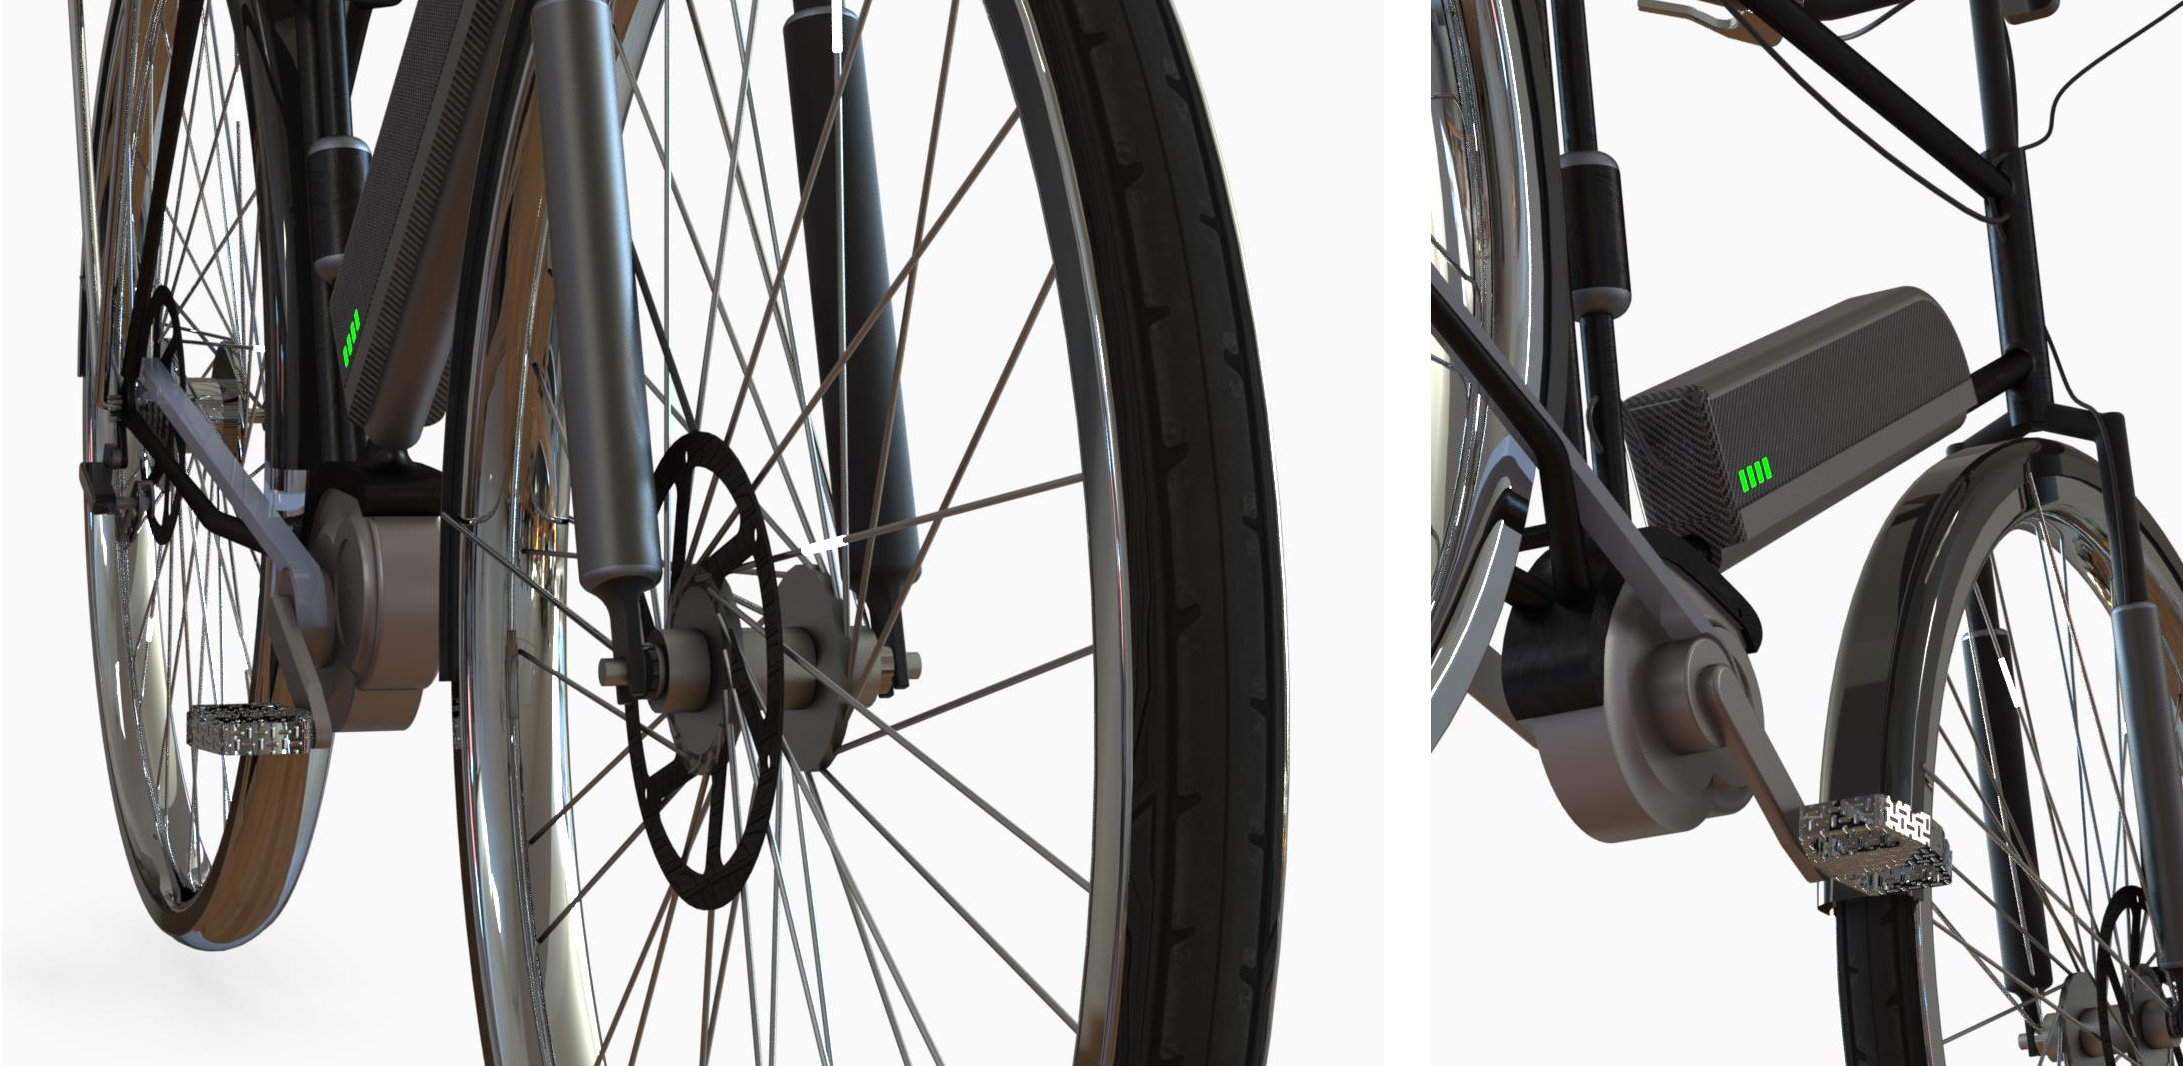
\includegraphics[width=0.98\textwidth]{bikeclose}
	\caption{Close-ups of integrated features}
\end{figure}


\subsection{Component Selection}
\label{sec:comps}

The following component selection was divided between: suspension, electrical drivetrain, and further components.

\subsubsection{Suspension Selection}

It was decided that the design would incorporate a fully suspended bike for two reasons. The first of them, was the fact that incorporating electrical components could increase the weight by up to 25 kilograms. Secondly, reducing the vibrations acting on these electrical components will prolong their lifetime \cite{muetz07}.

The choice for the front suspension was quite simple. The team decided to go forward with a classical front fork suspension system. This is simple, affordable, and efficient. Since the design was not intended for a performance bike, the required system needed only to fit two criteria: quality and affordability. Following these guidelines, the team chose the \textbf{SR Suntour XCR-RL Fork Suspension}. This choice was made based on the reliability of the company and the specifications detailed for the specific product \cite{suntour}. 

However, a design problem was encountered when considering the rear suspension. Most available rear suspension designs are made for high-performance bicycles such as mountain bikes. These types of bicycles often have ``futuristic'' and ``sporty'' frames. This was a problem because the design had to incorporate rear suspension into a classical frame; something which isn't too common in the industry. After considering a series of suspension designs, it was determined that a Horst-link (four-bar) design would be incorporated \cite{stott}. This decision was made for two reasons: the Horst-link was one of the few designs which had some similarity to the specific frame choice, and it left lots of options for suspension designers when considering values such as the instant centre (IC), anti-squat, pedal kick-back, and anti-rise.

The Horst-link design is a suspension design where the rear axle is indirectly connected to the main frame via a system of pivot points which allow the rear wheel to compress the dampener. As the dampener compresses, the rear axle moves upwards relative to the static main frame. A basic example of this design is shown below in Figure~\ref{fig:hor}.

\begin{figure}[!ht]
	\centering
	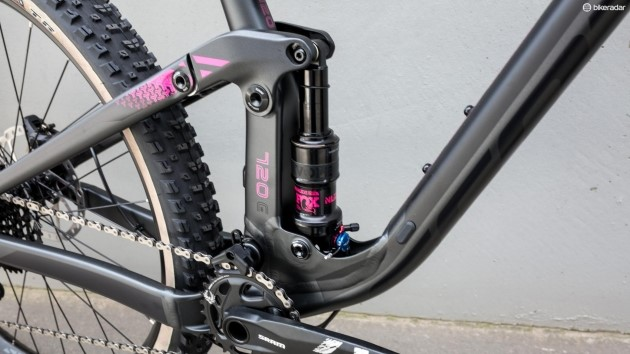
\includegraphics[width=0.8\textwidth]{horst}
	\caption{Conventional Horst-Link design}
	\cite{stott}
	\label{fig:hor}
\end{figure}

A few differences may be noted between the frame required for a conventional Horst-link design and the team's frame of choice. There is a difference in the angle of orientation of the top rear axle between both designs. In the end design, the frame requires a significantly greater angle. However this is not a problem, as this can be altered, and the dampener can be set beneath the seat. The orientation of the top axle will be selected such that it appears to be a continuation of the horizontal bar of the main frame. Due to the small dimensions of the dampener, this will not affect the ease of mounting and dismounting the vehicle. 

Furthermore, the design in Figure~\ref{fig:hor} has two predominant pivot points: at the connection to the main frame and the connection to the dampener. However, due to the increased geometry of the pedals due to the incorporation of the electric motor, another crucial pivot point must be incorporated at the pedal clearance. This will enable the whole of the rear axle to move in a circular fashion around this connection point; with the positioning being dictated by the dampener compression. Additionally, the dampener will have to be relatively stiff to avoid substantial deflections, as this would not go well together with a classic frame. 

The final integration into the design, modelled in CAD, is shown below.

\begin{figure}[ht]
	\centering
	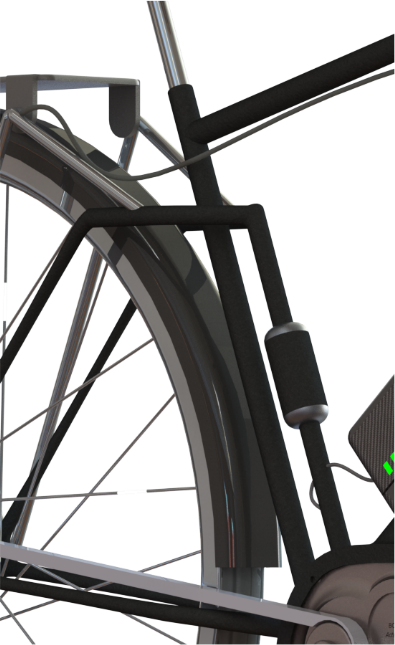
\includegraphics[width=0.4\textwidth]{ourhor}
	\caption{Rear suspension integrated into a classic bike frame (using SolidWorks)}
	\label{fig:ourhor}
\end{figure}

\newpage

In terms of the selection of the dampener, the same criteria applies as for the front suspension: a quality product with a requirement of average performance. For this purpose, the team decided to go with the \textbf{M2R Rear Shock Absorber 270mm} due to its reputation in the market, performance, and reduced dimensions \cite{m2r}. 

\subsubsection{Electrical Drivetrain Selection}

When considering the electrical drivetrain, the first decision was to decide on the type of motor to be incorporated into the design. The available options where: AC motors, DC motors, and brushless DC (BLDC) motors. AC motors are rarely used within the electric bicycle market due to the requirement of inverters for converting AC to DC, which add extra mass. However, the market is split when it comes to selecting between a DC and BLDC motor. 

When comparing both, BLDC motors prove to require a greater investment due to being more complicated, however, they are quieter, more powerful, and last longer. Furthermore, DC motors are not good at constant speed control. Keeping in mind the project's target quality, and the fact that it is designed for city use, where a good constant speed control is necessary, the team decided to proceed with a BLDC motor \cite{rag14}. 

Once the type of motor was selected, the following step was to consider where the motor would be mounted onto the frame. As specified in the morphological analysis, the following options were considered: frame mounted motor, hub motor, and belt-drive. Upon simple consideration and market analysis, this extensive list was narrowed down to two options: frame mounted and hub motors. 

Initially, hub motors were given preference due to their simplicity, as they required no interaction with the primary chain; leading to minimal maintenance. However, hub motors contribute towards the total un-sprung weight of the vehicle. Un-sprung weight increases rotational inertia, which negatively impacts the acceleration and driving dynamics of the vehicle \cite{fen13}. This could be fixed by using high-tech materials, such as composites, for the wheel and rim; nonetheless, the team decided to go with the simpler option to avoid unnecessary complications. Therefore, a frame mounted motor was chosen. These motors provide good power transfer without complications but require an additional chain and planetary gears which increase the sprung weight of the vehicle \cite{rag14}. 

When it came to motor power selection, not much design freedom was left, as EU standards set the maximum power to 250W \cite{15194}. A more powerful motor requires a battery with a greater capacity. However, the usage of a 250W motor within the EU market is standard within the industry, with very few products offering less powerful motors. Furthermore, one of the leading user requirements was to provide a vehicle which would enable a man to commute to work without arriving sweaty. Therefore, a powerful motor will require minimal physical effort. Hence, despite this requiring a battery with a greater capacity, a 250W motor was chosen. 

Following the previous characteristic specifications: 250W BLDC frame mounted motor, the team analysed the market for potential candidates. The electric bicycle motor market is segmented between Bosch, Yamaha, Shimano, and Panasonic. Upon inspecting the brand reputations, and the products they offered, a clear candidate rose: Bosch. 

First, Bosch is the most common electric bicycle motor brand, and its past and future performance have moulded a reputation of quality and reliability. Furthermore, Bosch has a branch of motors which have been optimised for city use: Bosch's Active Line. Within this line, the company offers the Active Line, and Active Line Plus, with the only difference being a greater initial torque in the latter. Since motor acceleration is not essential within city use (most of the driving will take place at constant speed), \textbf{Bosch's Active Line} was chosen. Furthermore, the motor offers four different driving modes, which include city optimisation and efficiency, giving the user greater freedom when choosing his desired driving experience. The selection is shown in the Figure~\ref{fig:bosmot} \cite{bosch18}.

\begin{figure}[!ht]
	\centering
	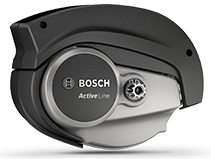
\includegraphics[width=0.4\textwidth]{bosmot}
	\caption{The chosen 250W BLDC frame-mounted motor -- Bosch's Active line}
	\cite{bosch18}
	\label{fig:bosmot}
\end{figure}

When considering the rest of the electrical drivetrain, an early decision was made to select components from Bosch. This would ensure a highly compatible drivetrain with full warranty, which would further simplify design and possibly result in greater cost reductions when bulk ordering. When considering the battery, many possibilities were present, including: lead-acid (sealed), lithium-ion, NiCd, and NiMH. However, after looking at the advantages and disadvantages of each, the team decided to follow the industry standard: Lithium-ion \cite{rag14}. 

As the vehicle would be used for commuting to work and back within the city, it was deemed that the required range was not too big. First, charging ports are generally available at both work and home. Furthermore, commutes within the city are not expected to be too big. Therefore, it was deemed that a range of 40 km would be adequate. Using Bosch's provided battery performance, shown in Figure~\ref{fig:crura}, a selection of a \textbf{300Wh Lithium-ion battery} (rechargeable in 3.5 hours) was made, along with the corresponding Bosch charger \cite{bosch18}.

\begin{figure}[ht]
	\centering
	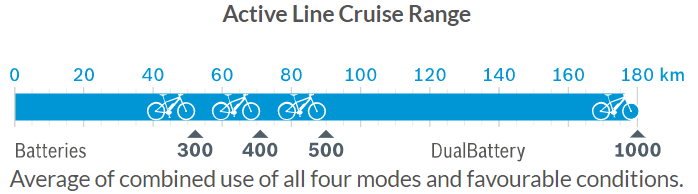
\includegraphics[width=0.8\textwidth]{crura}
	\caption{Active Line cruise range information provided by Bosch}
	\cite{bosch18}
	\label{fig:crura}
\end{figure}

\subsubsection{Further Selection}

The previous two components (electrical drivetrain, and suspension) have resulted in most of the available budget being invested into them, as will be shown in the cost analysis (Section~\ref{sec:coim}). Therefore, to keep costs within the target range specified in the PDS, the rest of the component selection has been carried out keeping the following criteria in mind: 

\begin{itemize}
	\setlength{\itemsep}{0pt}
	\item Other components require only basic performance.
	\item Selected component must still offer high quality.
	\item Selected brand must have a good reputation within their market.
\end{itemize}

The frame, wheel, and wheel hub were designed in house due to these components being relatively simple to manufacture. In house design guarantees quality on top of reducing costs. Further information regarding the material selection for these components is provided in the following section (\ref{sec:matse}). However, other components such as tyres, seats, handlebars, chains, and headlights are too specialised to manufacture. Therefore, these will be purchased from external suppliers, which are specialised and experienced. 

\begin{enumerate}[leftmargin=0pt, itemindent=20pt,labelwidth=15pt, labelsep=5pt, listparindent=0.7cm,align=left]
	\item Tyres:
		
		Schwalbe tyres were selected due to the company's experience and reputation within the bicycle market. The brand offers tyres, which have been specifically designed for city use. Furthermore, their tyres can be purchased optimised for e-bikes; improving driving dynamics. Therefore, the investment was made into their tyres, specifically, \textbf{Schwalbe Marathon GreenGuard City 26''} tyres \cite{schwalbe18}. 

	\item Seat:

		For the seat, the PDS required a leather comfort saddle, which will further improve the user's driving experience and comfort. For this purpose, the \textbf{Bioflex Websprung Gents Comfort} saddle was chosen because it fulfils the PDS, is designed specifically for men, and offers a cost-effective solution which remains visually appealing \cite{bioflex18}. 

	\item Handlebar:

		Similarly, the handlebar had to offer comfort and integrate into the rest of the bicycle design. For this purpose, the \textbf{Raleigh RNH361 Trekking Comfort Handlebar -- Silver} was selected. A special request will have to be made when purchasing this product, as the design requires leather grips. This slightly larger investment will result in both leather seats and handlebar grips: an iconic look for classical bikes \cite{raleigh18}. 

	\item Brakes:

		The morphological analysis required disc brakes, because rim bakes are not sufficient for electric bicycles due to the increased weight from the electrical drivetrain. However, within the range of available disc brakes, the cheapest ones will be sufficient for city use. Therefore, Clarks Cycle Systems have been selected as a provider due to their experience and reliability. Specifically, the \textbf{Clarks CMD-11 Mechanical Disc Brake + Rotor} have been chosen for the design \cite{clarks18}. 

	\item Other:

		Further non-crucial components have also been specified for the design, however, due to their low importance, no explanation has been given regarding the choice. Nonetheless, it can be noted that \textbf{Shimano components} were frequently selected due to the company's size and experience within the general bicycle market \cite{shimano18}. The following table provides a list of the chosen components.
\end{enumerate}

\begin{table}[!ht]
	\centering
	\caption{Defined non-crucial bicycle components}
	\begin{tabular}{l l}
		\hline
		Bike component&Component choice\\ \hline
		Chain 	&Shimano HG93 (9 speed) Roller Chain \\
		Headlight	&Bobbin Retro Front Light \\
		Bolts	&Stainless Steel Thread Hexagon Bolts\\
		Pannier rack	&Tortec Velocity Rear Pannier Rack - Silver\\
		Brake handles	&Shimano BL M425 Acera Complete Brake Lever\\
		Mudguards	&SKS Bluemels Mudguard Set \\
		Cables	&Shimano PTFE Coated Stainless Steel Inner Wire 
	\end{tabular}
\end{table}


\subsection{Material Selection}
\label{sec:matse}

Throughout most vehicle markets, the predominantly used materials are: titanium, steel, and aluminium. In general, titanium is an expensive material, which offers the best strength to density ratio. Aluminium is an affordable material, which offers a good strength to density ratio. And finally, steel is the cheapest option, offering the worst strength to density ratio. A visual comparison of the three materials is offered in Figure~\ref{fig:cpuc} below. 

\begin{figure}[ht]
	\centering
	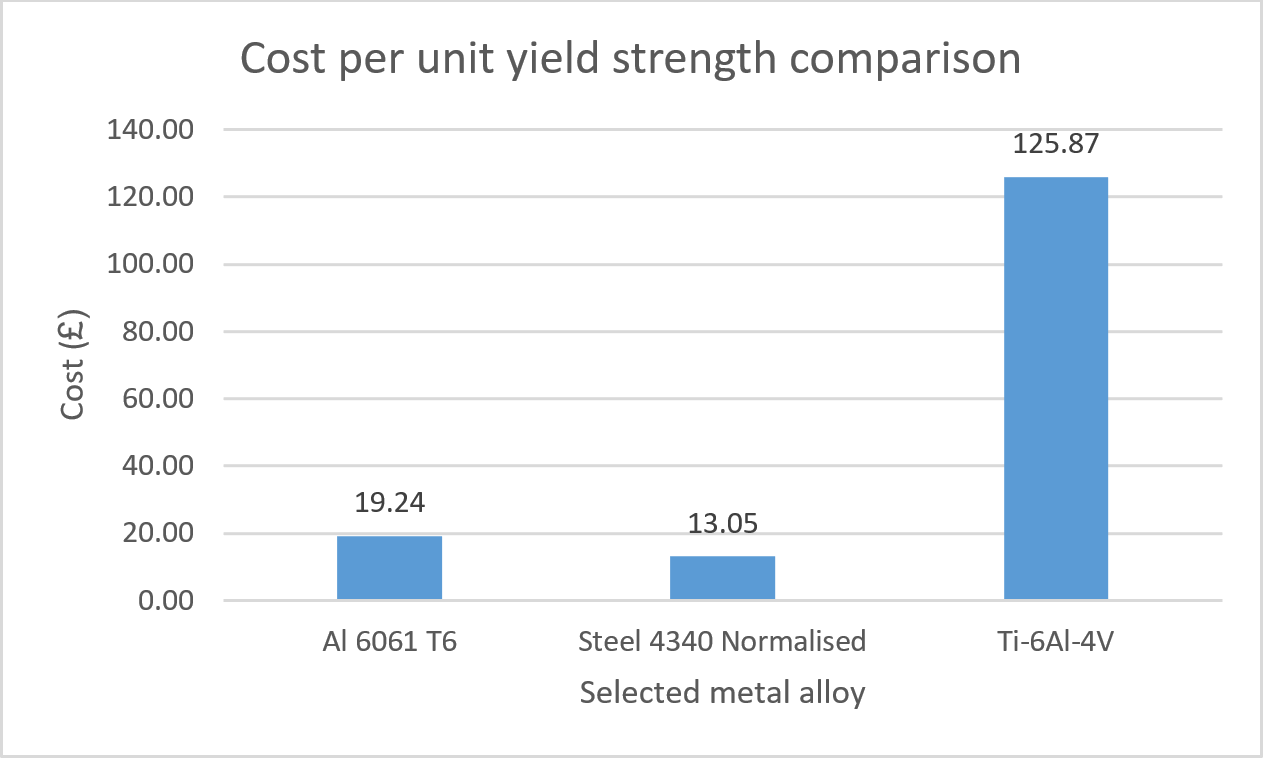
\includegraphics[width=0.8\textwidth]{cpuc}
	\caption{Comparing the cost in pounds per unit yield strength for specific metals used within the vehicle industry. Values used are not specific for alloys, but rather an average of the material itself.}
	\cite{CES}
	\label{fig:cpuc}
\end{figure}

The intended use of the electrically assisted bike is within the city; therefore, the components will not demand any significant performance. As mentioned previously, a great investment was made into two components, therefore, the material selection must be done by trying to keep costs at a minimum whilst maintaining quality and reliability. Keeping this in mind, titanium was disqualified as it is used in expensive high-performing bicycles. Although aluminium is more expensive than steel (usually 150\% the price), it was determined that it was an acceptable investment due to the increased strength to density ratio. Furthermore, aluminium is also more cost effective when considering both Young's modulus and the elastic modulus. The aluminium used for specific components will be discussed in the following sections. 

Throughout the following processes, data and prices were extracted from CES software \cite{CES}. Any other sources will be clearly referenced. 

\subsubsection{Frame}

From preliminary market analysis, it was determined that the most common alloys used for the frame were 6061-T6 aluminium and 7005-T6 aluminium. The T6 temper was chosen for both alloys due to its cost-effective enhancement, 7005-T6 is used in less expensive frames. It has very similar properties to 6061-T6, with the primary difference being 6061-T6's reduced density (2700 kg/m3 as opposed to 2780 kg/m3) \cite{mif}.  Additionally, 7005-T6 does not have to be precipitation hardened, it is simply air hardened. 

It was decided that the slight density advantage offered by 6061-T6 over 7005-T6 did not justify the larger investment. Furthermore, 7005-T6 has an ease of welding and manufacture. Therefore, the bike frame will be made up of welded \textbf{7005-T6 Aluminium} pipes. Specifically, gas metal arc (MIG) welding was chosen due to its low cost, simplicity, and material compatibility. Unfortunately, 7005-T6 is susceptible to corrosion; therefore, the paint coating will have to include anti-corrosive properties, slightly increasing the cost of the paint. 

\subsubsection{Wheel and Hub}

Due to the specific geometries of the wheel and hub, the material selection process gave priority to the manufacturing properties, rather than the mechanical properties. The simplest method of manufacturing the wheel and hub is through casting. Upon some preliminary research, it was determined that cast aluminium was the best for this purpose, specifically \textbf{AlSi10Mg} due to its superior mechanical properties. AlSi10Mg will be used for both the wheel and the hub. Furthermore, low-pressure die-casting has been chosen for manufacturing due to its low cost, high material compatibility, and scalability. 

\subsection{Calculations}
\label{sec:calculations}

In order to accomplish a functioning bicycle, apart from measurements based on the adult male body, the exact centre to centre distance, and preliminary force calculations were considered.

\subsubsection{Centre to centre distance}

To determine the exact centre to centre distance, the following values were defined:

\begin{itemize}
	\setlength{\itemsep}{0pt}
	\item Estimated power output over the length of the commute at: 200W \cite{wilson04} 
	\item Number of teeth in the block, $N_{1}$: 12 (based on design) 
	\item Number of teeth in the chain ring, $N_{2}$: 36 (based on design) 
	\item Smooth running and an application factor of: 1 \hfill\cite{childs04}
	\item Selection rating based on a 19 tooth sprocket \hfill\cite{childs04}
	\item Centre to centre distance, $C$: 490mm (based on design) 
	\item Cycling at a leisurely cadence of: 70RPM \hfill\cite{lucia01}
\end{itemize}

This gives a selection power of 316.67W, calculated with the following equation:
\begin{gather*}
	\text{Selection Power}=\text{Estimated Power Output}\times\text{Application Factor}\times\text{Tooth Factor}\\
	316.67\text{W}=200\text{W}\times 1\times \frac{19}{12}
\end{gather*}

Next, in order to select chain pitch, the driver sprocket speed is determined:
\begin{gather*}
	\text{Driver Sprocket Speed}=\text{Cadence}\times\text{Reduction Ratio}\\
	210\text{RPM}=70\text{RPM}\times\frac{36}{12}
\end{gather*}

As a result, taking selection power and driver sprocket speed, for a 19 tooth drive sprocket, the chain pitch length, $p$, is determined to be: 8mm \cite{childs04}.

With the chain pitch length and the determined values of the design, based on the number of pitches, the chain length is determined to be:
\begin{gather*}
	\text{Number of pitches}=\frac{N_{1}+N_{2}}{2}+\frac{2\times C}{p}+\left(\frac{N_{2}-N_{1}}{2{\pi}}\right)^{2}\times\frac{p}{C}\\
	146.738=\frac{36+12}{2}+\frac{2\times 0.490}{0.008}+\left(\frac{36-12}{2{\pi}}\right)^{2}\times\frac{0.008}{0.490}\\
	\text{Number of Pitches:}\quad L=147\ \text{(rounded up)}
\end{gather*}

Giving an exact centre to centre distance ($C$) of:
\begin{gather*}
	C=\frac{p}{8}\left[2L-N_{2}-N_{1}+\sqrt{\left(2L-N_{2}-N_{1}\right)^{2}-\frac{{\pi}}{3.88}\left(N_{2}-N_{1}\right)^{2}}\,\right]\\
	C=\frac{0.008}{8}\left[2\times 147-36-12+\sqrt{\left(2\times 147-36-12\right)^{2}-\frac{{\pi}}{3.88}\left(36-12\right)^{2}}\,\right]\\
	\text{\textbf{Exact Centre to Centre Distance}}=491.050\,\text{mm}
\end{gather*}

This value, given by the equations from \textit{Mechanical Design} by Childs, is only 1.05 mm from the intended design distance. It also demands manual lubrication, which is a typical method of lubrication for bicycles.

\subsubsection{Force Calculations}

In order to quantify the performance of the bicycle in operating conditions, calculations were carried out based on each individual member. The calculations were performed by inspecting each member and applying a force comprised of a 120 kg rider, and the total bicycle weight based on the design (24.663 kg). This resulted in a total force of 1419.144N. 

In Table~\ref{tab:fo}, the properties of the member: outer radius ($r_{o}$), inner radius ($r_{i}$, blank if the member is hollow), and member area ($A$) are defined. Furthermore, the maximum stress (${\sigma}_{max}$) describes the maximum stress that is applied when the entire mass of the rider and bicycle, are applied to the member. This value serves as an extreme condition, which the bicycle should ideally be able to withstand. Lastly, (${\sigma}$) serves as an estimated real stress value, that varies based on the percentage of total force that is applied to the member (percentage is indicated next to each value of ${\sigma}$).

\begin{table}[!ht]
	\centering
	\caption{Force Calculations}
	\begin{tabular}{l r r r r r r}
		\hline\\[-2ex]
		Member Type&\multicolumn{1}{c}{$r_{o}$ (mm)}&\multicolumn{1}{c}{$r_{i}$ (mm)}&\multicolumn{1}{c}{$A$ (mm\textsuperscript{2})}&\multicolumn{1}{c}{${\sigma}_{max}$ (N/mm\textsuperscript{2})}&\multicolumn{1}{c}{${\sigma}$ (N/mm\textsuperscript{2})}&\multicolumn{1}{c}{\%}\\\hline
		Seat tube&10&8&113.097&12.548&5.647&45\\
		Down tube&10&8&113.097&12.548&5.647&45\\
		Top tube&10&8&113.097&12.548&5.647&45\\
		Head tube&15&10&392.699&3.614&1.626&45\\
		Forks&10&8&113.097&12.548&5.647&45\\
		Seat stay&6&&113.097&12.548&5.647&45\\
		Chain stay&6&&113.097&12.548&5.647&45\\
		Handlebars&10&&314.159&4.517&1.581&35\\
		Pedals&8&&201.062&7.058&1.412&20\\
		Seat connector&16&&804.248&1.765&0.749&45\\
		Upper seat connectors&10&&314.159&4.517&2.033&45\\
	\end{tabular}
	\label{tab:fo}
\end{table}

Given that the maximum stresses are all found to be below the material strength (310 MPa \\\cite{mif}), it can be concluded that the bicycle will be able to operate for its intended purpose.

\subsection{Standards Considered}
\label{sec:standard}

As mentioned in Section~\ref{sec:pds}, there are certain standards that must be considered in order to sell this design as a legal bicycle in Europe.

In regards to the electrical components, EN 15194 outlines electrical requirements, testing procedures, standard symbols, etc. \cite{15194}. The elements in the detailed design, must be in accordance with the contents of this standard, as it has been adopted by the European Union. Otherwise this product will not be recognised as an EPAC (electric pedal-assisted cycle). In that case, the design will require further licensing by the user and can't be sold as an e-bike, which in this case is undesirable.

In order for the bike to be considered safe in Europe, the bike must adhere to the standards in EN 14764. This document details all safety and testing specifications for all components of a conventional city bicycle \cite{14764}. This standard has also been adopted by the European Union and thus to reduce complications, the final product will comply to its requirements.

Relative to the manufacturing of this bicycle, all tolerances, limits, and fits will be in accordance with ISO 286. Therefore all fits that require a shaft or bearing (e.g. handlebar, seat-post, wheel hub, etc.), will have a specified tolerance sizing which promotes interchangeability and functionality in production \cite{286}.

Additional standards refer to the assembly mechanisms of the bicycle. This includes: qualification testing of welders in particular with aluminium \cite{9606}, appropriate cross recessed screws \cite{4757}, and appropriate hex keys \cite{4762}.

\section{Costing and Implementation}
\label{sec:coim}

As specified previously, in the Market Analysis (Section~\ref{sec:caac}), the goal price for this product was \textsterling 1,960. This price was extracted from the average price in the electric-city-bicycle market. The goal is to offer a high-quality product within this range, such that the designed electrical bicycle is economically competitive. It must be kept in mind that the market for classical looking e-bikes is underdeveloped, and therefore the product will also benefit from a smaller amount of competition.  

The costing was carried out following one principle assumption: the bike is being designed by a large company which is looking to penetrate the e-bike market. Therefore, many overheads such as hardware, software, and rent will not be considered. Although this may not represent the entirety of the costing behind the bike design, it does a better job of focusing on the costing of the engineering design itself rather than incorporating other external factors. The approach and equations used are the ones provided in the PowerPoint slides of the Mechanical Design 2 course.

Overall, the selling price was calculated using the formula below: 
\[
	\text{Selling Price} = \text{Profit Margin} \times \left(\text{Works Cost Price} + \text{Design Material} + \left(\frac{\text{Design Labour}}{\text{Quantity}}\right)\right)
\]

\subsection{Cost of Design Labour}

The cost of design represents the money invested into each bicycle in the forms of both the cost of research and development for designing the bicycle. Both the design labour costs have been calculated and are provided in Table~\ref{tab:labco} below.  

\begin{table}[!ht]
	\centering
	\caption{Specific and total design labour cost}
	\begin{tabular}{l r r r}
		\hline
		\multicolumn{1}{l}{Tasks}&\multicolumn{1}{l}{Hours (h)}&\multicolumn{1}{l}{Cost per Hour (\textsterling/h)}&\multicolumn{1}{l}{Total Cost (\textsterling)}\\\hline
		Developing PDS	&3&20.00&60.00\\
		Initial Research&20&20.00&400.00\\
		Market Analysis&6&20.00&120.00\\
		Component Selection&8&20.00&160.00\\
		Material Selection&6&20.00&120.00\\
		Morphological Analysis&3&20.00&60.00\\
		Biomechanical Analysis&5&20.00&100.00\\
		CAD&20&20.00&400.00\\
		Further Development&100&20.00&2000.00\\
		FEA Simulation&20&20.00&400.00\\
		Component Testing&200&20.00&4000.00\\
		Drive Testing&20&10.00&200.00\\\hline
		Total&411&&8020.00\\\hline
	\end{tabular}
	\label{tab:labco}
\end{table}

The hours necessary for the completion of tasks provided above, are based on approximations of the actual work invested by the team throughout the design process. Furthermore, a testing phase has been included in the design labour costs. 

Although testing in general is not expensive, it is very time intensive. Therefore, in certain situations this can lead to an accumulation of substantial costs. In this case, the testing was: 20 hours of CAD (computer aided design), 200 hours of mechanical component testing, and 20 hours of testing the final product in the environment of use. 

\subsection{Cost of Design Material}

The cost of design material was calculated and is provided in Table~\ref{tab:desmat} below. 

\begin{table}[!ht]
	\centering
	\caption{Specific and total design material costs}
	\begin{tabular}{l l r r}
		\hline
		\multicolumn{1}{l}{Component}&\multicolumn{1}{l}{Specification}&\multicolumn{1}{l}{Quantity}&\multicolumn{1}{l}{Total Cost (\textsterling)}\\\hline
		Motor&Bosch ActiveLine 250W BLDC&1&250.00\\
		Battery&Bosch Powerpack 300Wh (40 km range)&1&400.94\\
		Charger&Bosch Charger 4A&1&100.00\\
		Front Suspension&SR Suntour XCR-RL Fork Suspension&1&114.95\\
		Back Suspension&M2R Rear Schock Absorber 270mm&1&40.00\\
		Frame&7005-T6 Aluminium (Age Hardening) - 1500g&1&2.93\\
		Wheel&Cast Aluminium - 800g&2&3.12\\
		Tyre&Schwalbe Marathon GreenGuard City (26 in)&2&17.99\\
		Wheel Hub&Cast Aluminium - 300g&2&1.17\\
		Seat&Bioflex Websprung Gents Comfort&1&19.96\\
		Handlebar&Aluminium and Leather Coated&1&25.00\\
		Chain&Shimano HG93 (9 speed) Roller Chain&1&10.99\\
		Headlight&Bobbin Retro Front Light&1&19.99\\
		Brakes&Clarks CMD-11 Mechanical Brake Disc + Rotor&2&11.99\\
		Brake Handles&Shimano BL M425 Acera Brake Lever&2&14.44\\
		Cables&Shimano PTFE Coated Stainless Steel Wire&1&6.99\\
		Pannier Rack&Tortec Velocity Rear Pannier Rack - Silver&1&21.59\\
		Mudguard&SKS Bluemels Mudguard Set&1&25.38\\\hline
		Total&&&1087.43\\\hline
	\end{tabular}
	\label{tab:desmat}
\end{table}

The components included in this table are the ones mentioned previously in the Component Selection (Section~\ref{sec:comps}). The prices for the raw materials used for the frame, wheel, and wheel hub have been obtained from CES software. Retail prices have been considered for the components not being manufactured. This means that the situation being considered is a worst-case scenario. The total cost could be expected to drop anywhere from 10\% to 20\% if wholesale prices were obtained from the providers. 

\subsection{Works Cost Price}

Works cost price considers the costs of manufacturing and assembling every bicycle. This includes both the cost of processes, and the salaries of the workers completing these processes. The manufacturing processes considered are the ones selected in the component selection section. Time has been allocated for the mechanical assembly and electrical wiring of the bicycle. Furthermore, an additional 2 hours of mechanical testing of each bicycle has been included. This testing process could comprise of fastener testing, suspension testing, and overall performance; in order to accommodate the needs of any standards mentioned in Section~\ref{sec:standard}. 

\begin{table}[!ht]
	\centering
	\caption{Specific and total works cost price per bike}
	\begin{tabular}{l r r r}
		\hline
		\multicolumn{1}{l}{Process}&\multicolumn{1}{l}{Hours (h)}&\multicolumn{1}{l}{Cost per hour (\textsterling/h)}&\multicolumn{1}{l}{Total Cost (\textsterling)}\\\hline
		Mechanical Assembly&2&15.00&30.00\\
		Electrical Wiring&1&15.00&15.00\\
		Gas Metal Arc (MIG) Welding&1&30.00&30.00\\
		Low Pressure Die Casting&1&5.00&5.00\\
		Testing&2&20.00&40.00\\\hline
		Total&7&&120.00\\\hline
	\end{tabular}
\end{table}

\subsection{Final Cost}

The retail price was calculated assuming a worst-case scenario where only 100 e-bikes are sold within the first year. Throughout several iterations it was determined that the highest profit margin that could be applied whilst maintaining the price within the specified target, was 50\%. This is a healthy profit margin, which enables the business to grow and reinvest a portion of their profit into further research and development to remain competitive. The calculated price is shown below: 
\[
	\text{Selling Price} = 1.5 \times \left(1087.43+120.00+\frac{8020.00}{100}\right) =\text{\textsterling}1,931.45
\]

With a cost of production of \textsterling 1,287.63, this leads to a total profit of \textsterling 643.82 per bike. This price is slightly below the product price target that was set previously. Therefore, the goal of providing a quality product whilst maintaining industry standard prices has been accomplished throughout the design phase. Furthermore, a couple more factors must be kept in mind. 

The figures obtained above have not considered wholesale prices or economies of scale. Therefore, the price could be expected to decrease by up to 30\%. Nonetheless, it has been proven that the current design is economically viable. Therefore, the final selling price can be determined once prices are consulted with retailers, further market analysis is conducted, and focus groups are carried out to understand the current market tendencies.  

\subsection{Break Even Analysis}

Using the costs and prices laid out in the previous sections, a break-even analysis was conducted. It was assumed that for the given production capacity of 100 units per year, there would be three employees working full time at a standard wage of \textsterling 23,333.00 per year. The graph for the break-even analysis is provided in Figure~\ref{fig:roi} below.

\begin{figure}[!ht]
	\centering
	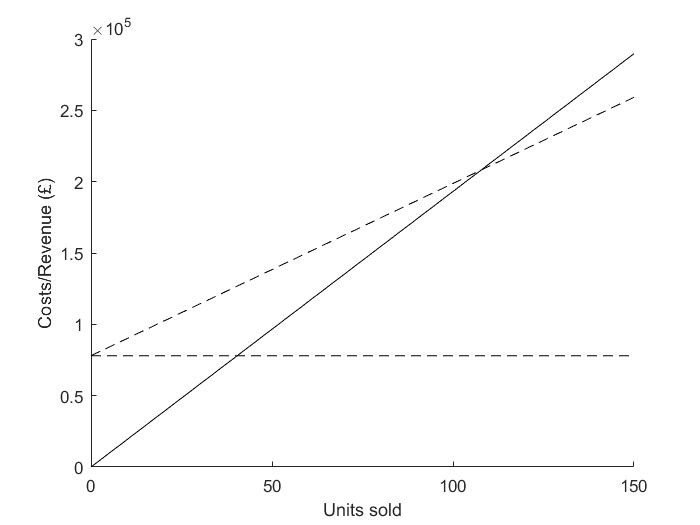
\includegraphics[width=0.8\textwidth]{geg2}
	\caption{Costs are represented by the dotted line, and revenue by the full line. Break-even achieved after 108 units sold.}
	\label{fig:roi}
\end{figure}

As obtained from the graph, the break-even is achieved after 108 units are sold. The final pricing calculation was conducted assuming that only 100 bikes were sold in the first year. Although it was mentioned that this was a worst-case scenario, there seems to be a slight discrepancy as the break-even point is greater than the units assumed to be sold. This problem was further assessed by conducting profit and loss accounts in the following section. 

\subsection{Profit and Loss Accounts}

The profit and loss accounts have been created for the first three years of the forecasted sales. Three different expected sales have been considered throughout the years, these are 100, 1,000, and 10,000. A profit and loss account has been calculated for each one of them. 

For each scenario, the same rounded selling price of \textsterling 1,930.00 was used, despite it being calculated only for the 100 units sold scenario. This provided some consistency throughout the three considered scenarios. It was assumed that the number of full time employees required to manufacture 100 bicycles per year were 3, each having a salary of \textsterling 23,333 per annum (total of \textsterling 70,000). 30 were required for 1,000 bicycles (total of \textsterling 700,000), and 300 for 10,000 bicycles (total of \textsterling 7,000,000). 

Furthermore, the first year presented two extra costs. The first was a design labour cost of \textsterling 8,200 and the second was a cost of tooling of \textsterling 100,000. Both are paid off in the first year and from then on, do not appear again in the profit and loss account. Taking a conservative approach, a contingency of \textsterling 10,000 was included for every 100 bicycles produced. Finally, a 20\% discount off raw materials was assumed for the 1,000-purchase scenario, whilst a 30\% discount was assumed for the 10,000 units scenario. The profit and loss accounts are shown in Table~\ref{tab:PLA} below. 

Due to the healthy, and comfortable, 50\% profit margin imposed on the selling price, only three of the nine considered years would result in economic loss, with two of them being a minimum loss of \textsterling 7,743.00. 

\begin{table}[!ht]
	\centering
	\caption{Expected Profit and Loss accounts for units sold over the first three years}
	\begin{tabular}{l r r r r r r}	
		\hline
		Profit \& Loss Account Y1&\multicolumn{1}{l}{No.}&\multicolumn{1}{l}{\textsterling}&\multicolumn{1}{l}{No.}&\multicolumn{1}{l}{\textsterling}&\multicolumn{1}{l}{No.}&\multicolumn{1}{l}{\textsterling}\\ \hline
		Units Sold at \textsterling 1,930.00&100&193,000.00&1,000&1,930,000.00&10,000&19,300,000.00\\
		Costs of Sales at \textsterling 1,207.43&&120,743&&965,944&&8,452,010\\
		Total Direct Costs&&78,020.00&&708,020.00&&7,008,020.00\\
		Gross Margin&&-5,763.00&&256,036.00&&3,839,970.00\\
		Contingency (with tools)&&110,000.00&&200,000.00&&1,100,000.00\\
		Net Profit/Loss before Tax&&-115,763.00&&56,036.00&&2,739,970.00\\
					  &&&&&&\\ \hline
		Profit \& Loss Account Y2&\multicolumn{1}{l}{No.}&\multicolumn{1}{l}{\textsterling}&\multicolumn{1}{l}{No.}&\multicolumn{1}{l}{\textsterling}&\multicolumn{1}{l}{No.}&\multicolumn{1}{l}{\textsterling}\\ \hline
		Units Sold at \textsterling 1,930.00&100&193,000.00&1,000&1,930,000.00&10,000&19,300,000.00\\
		Costs of Sales at \textsterling 1,207.43&&120,743&&965,944&&8,452,010\\
		Total Direct Costs&&70,000.00&&700,000.00&&7,000,000.00\\
		Gross Margin&&2,257.00&&264,056.00&&3,847,990.00\\
		Contingency&&10,000.00&&100,000.00&&1,000,000.00\\
		Net Profit/Loss before Tax&&-7,743.00&&164,056.00&&2,847,990.00\\
					  &&&&&&\\ \hline
		Profit \& Loss Account Y3&\multicolumn{1}{l}{No.}&\multicolumn{1}{l}{\textsterling}&\multicolumn{1}{l}{No.}&\multicolumn{1}{l}{\textsterling}&\multicolumn{1}{l}{No.}&\multicolumn{1}{l}{\textsterling}\\ \hline
		Units Sold at \textsterling 1,930.00&100&193,000.00&1,000&1,930,000.00&10,000&19,300,000.00\\
		Costs of Sales at \textsterling 1,207.43&&120,743&&965,944&&8,452,010\\
		Total Direct Costs&&70,000.00&&700,000.00&&7,000,000.00\\
		Gross Margin&&2,257.00&&264,056.00&&3,847,990.00\\
		Contingency&&10,000.00&&100,000.00&&1,000,000.00\\
		Net Profit/Loss before Tax&&-7,743.00&&164,056.00&&2,847,990.00\\
	\end{tabular}
	\label{tab:PLA}
\end{table}

\subsection{Return on Investment}
\label{sec:roi}

The return on investment (ROI) has been calculated for each year of each of the three expected sales scenarios. The ROI was conducted considering a cumulative approach. This meant that both the investment and profit calculated from year 1 are carried on into year 2. Therefore, the investment and profit in year 2 are equal to the sum of the investment and profit in year 1 and year 2, respectively. Similarly, year 3 considers the effect of the product on the business throughout all three years. For each year, the ROI was calculated as a ratio of profit to investment.  The results are shown in Table~\ref{tab:ROI} below. 

\begin{table}[!ht]
	\centering
	\caption{Cumulative ROI over the first three years of product launch}
	\begin{tabular}{r r r r}
		\hline
		\multicolumn{1}{l}{Year}&\multicolumn{1}{l}{100 Units Sold ROI}&\multicolumn{1}{l}{1,0000 Units sold ROI}&\multicolumn{1}{l}{10,000 Units sold ROI}\\ \hline
		1&0.6251&1.0299&1.1655\\
		2&0.7576&1.0605&1.1693\\
		3&0.8152&1.0711&1.1705\\
	\end{tabular}
	\label{tab:ROI}
\end{table}

The scenario where 100 bikes are sold never becomes profitable. The ROI does improve significantly over the first three years, however, from then on it will tend to a value slightly less than One over the following years. Therefore, this scenario would require a slightly higher profit margin. 

Conversely, the 1,000 bikes sold scenario has a steady increase in ROI, which although not great, still accounts for a 7.11\% improvement over the first three years. Therefore, the selling price is well selected for this situation. 

On the other hand, the 10,000 units sold scenario has a very large initial ROI with a slight increase over the years. Therefore, the profit margin could be decreased to attract more customers and establish the brand better within the market.

\subsection{Conclusion}

Although many assumptions have been made throughout the cost analysis section, worst-case scenarios were constantly considered throughout. Therefore, in practice, most costs could be expected to decrease, and the ROIs to improve. Meaning that even the 100 units sold scenario could become profitable. Nonetheless, it is important to conclude that this analysis showed that the design is economically viable. Although the selling price is not fixed, it has met the target selling price and quality goal; meaning that final and more refined selling prices can be implemented after further market and economic analysis. 

\section{Project Evaluation}

\begin{figure}[ht]
	\centering
	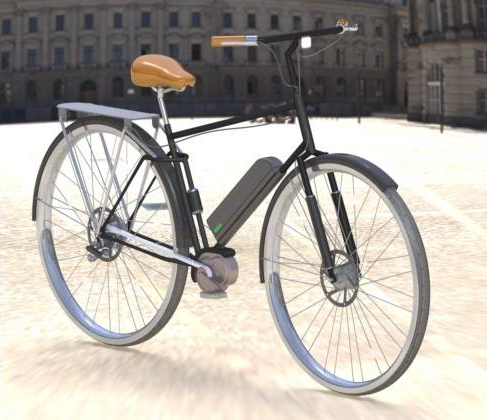
\includegraphics[width=0.8\textwidth]{dd}
	\caption{Final design in the city (rendered in SolidWorks)}
\end{figure}

\subsection{Detailed Design Analysis}

Referring to the initial product design specifications in Table~\ref{tab:pds}, a comparison between the final design and its features can be made.

\begin{enumerate}[leftmargin=0pt, itemindent=20pt,labelwidth=15pt, labelsep=5pt, listparindent=0.7cm,align=left]

	\item Technical Requirements:

		The use of Bosch's full electric bike components allows the final design to support intended purposes regarding power, without exceeding regulations set by the EU. The positioning of these components enhances the mobility of the bike, despite its increased weight. Additionally the selected frame design and material are proven reliable, and are able to accommodate the essential needs of the target businessman.
		
	\item Ergonomics:

		Comfort handlebars in combination with an upright riding style, provide a relaxed position (see Section~\ref{sec:biomech}) that is familiar to a conventional push bike. Furthermore, the added adjustability in the seat and handlebar, allows the bike to conform to a wide range of users appropriately. Finally, the Bosch components are sensibly integrated into the frame such that they do not hinder the user, whilst remaining convenient in the user's everyday work life.

	\item Maintenance:

		With Bosch components, the target user within the EU will be able to find expert mechanics, and replacements of any electrical equipment when necessary. Additionally, by adhering to assembly standards stated in Section~\ref{sec:standard}, the bulk of the bike remains easily maintained by conventional bike mechanics.

	\item Safety:

		By adopting European safety standards for city bicycles and e-bikes (Section~\ref{sec:standard}), the user will only require the suggested safety equipment (helmet). Therefore, the bike remains as safe on the road as any other typical bicycle on the market.

	\item Cost:

		With an estimated retail price of \textsterling 1,930, the bike remains below the market average (see Section~\ref{sec:runc}). Additionally given that the bike's design remained fairly conservative, the general maintenance cost is projected to be relatively low. Thus by taking these measures into account, the bike offers a well adjusted investment regardless of the user's location in Europe.

\end{enumerate}

\subsection{Merits and Improvements}

The merits of the design are its ease of use/maintenance. Given its similarities to a conventional bike, bike mechanics for the mechanical components can be easily sourced, due to the utilisation of market available components. The design is also heavily concerned with the comfort of the user during intended use, this means that the brief is fully fulfilled. The user will not overexert themselves, and will experience no discomfort, provided that the seat and handlebars are set up correctly. The design also has a factor of safety above what would be deemed necessary, as even when used under extreme conditions of loading (Section~\ref{sec:calculations}), it remains functional due to the material selection and geometry of the frame. The costing of the design also makes it very appealing to the market, as it is on the affordable side of city designed e-bikes, while tailoring specifically to businessmen.

Some improvements could be made to the design, concerning the cumulative ROI that becomes profitable at 1000 units minimum (Section~\ref{sec:roi}). However, as sales of e-bikes are increasing as seen in the market analysis (Section~\ref{sec:CAA}), the issue would correct itself; but for company financial security, it would be desired that fewer units are to be sold to break-even by increasing the profit margin. 

Another issue presents itself with the use of Bosch parts. While useful in terms of convenience as a manufacturer, they do come with issues as their parts are propriety. This causes most of the cost to to be allocated to these components, and reduces the potential freedom the user may have with his bike. If these components could be designed and manufactured in-house instead of relying on Bosch, the price of the product could be decreased in the long term, for a high up-front cost. Conversely, a cheaper alternative to Bosch could be sourced instead. These improvements would also help to solve the previously mentioned issues of break-even sales. 


\section{Group Work Analysis}

When the task was first commissioned, the team first met to discuss possible leadership roles, allocate work, and establish a method of communication. It was agreed that the leadership style would be decentralised with work progression and allocation relying heavily on group meetings, which had been scheduled once per week. In these meetings, the group members presented their work, discussed issues and ideas, and worked on sections of the project which required collaboration. This structure allowed constant feedback, in which every member took a role in decision making, and made sure that iterations in the design process remained fluid and constant. 

In terms of communication, it was determined that the most effective channel would be a Facebook group chat. Here, times for the weekly group meetings were discussed thoroughly. Furthermore, the team took advantage of the chat poll system and file exchange features to maintain project progression, and linearity throughout the week in a democratic manner. Once certain aspects of the project were finalised, these files were exchanged via a more formal channel of communication (E-mail). 

The biggest issue the team encountered, as reflected in Section~\ref{sec:fwa}, was scheduling meetings due to differences in timetabled classes. Nonetheless, the previously designed working framework allowed to override these complications. One of the first obstacles was the open-ended nature of the project. This required the group to create a very detailed PDS in order to lay down the groundworks for design to commence. Even though the PDS was very specific, with over 40 requirements, the team came up with too many possible designs. Therefore, the next issue, was honing these into a final design. This was accomplished through discussion of the pros and cons of the morphological analysis, followed by a voting process. Once these fundamentals were determined, the progress of the detailed design was smooth. However, when dealing with the PowerPoint presentation the team once again encountered minor issues with communication and workflow. These were amended via more frequent meetings on the run-up to the final presentation. These insights were helpful in preventing similar issues with the final report. 

Overall, the group members were satisfied with the way the project was carried out. If anything were to change for future endeavours, the group agreed that less time should be invested into initial research. In contrast, creating the PDS first, would allow more focused and efficient research to be conducted. 


\sloppy
\bibliographystyle{apacite}
\bibliography{References}


\nocite{shi}
\nocite{bosch16}
\nocite{sw}

\end{document}
